% ─────────────────────────────────────────────────────────────────────────────
%  AIMD Extended Profile v2.0: Technical Report
%  AI Model Distribution ODRL Profile for Training Pipeline Governance
%  MAI Dissertation, Trinity College Dublin, 2026
% ─────────────────────────────────────────────────────────────────────────────
\documentclass[12pt,a4paper]{article}

\usepackage[T1]{fontenc}
\usepackage[utf8]{inputenc}
\usepackage[margin=2.5cm]{geometry}
\usepackage{hyperref}
\usepackage{booktabs}
\usepackage{longtable}
\usepackage{tabularx}
\usepackage{array}
\usepackage{xcolor}
\usepackage{listings}
\usepackage{parskip}
\usepackage{microtype}
\setlength{\emergencystretch}{3em}
\usepackage{enumitem}
\usepackage{fancyhdr}
\usepackage{titlesec}
\usepackage{graphicx}
\graphicspath{{figures/}}
\usepackage{amsmath}

% ─── Colour palette ──────────────────────────────────────────────────────────
\definecolor{codeblue}{rgb}{0.0, 0.30, 0.60}
\definecolor{codegray}{rgb}{0.50, 0.50, 0.50}
\definecolor{compliant}{rgb}{0.09, 0.56, 0.19}
\definecolor{violation}{rgb}{0.80, 0.10, 0.10}
\definecolor{ttlbg}{rgb}{0.97, 0.97, 0.97}

% ─── Turtle / SPARQL listing style ───────────────────────────────────────────
\lstdefinelanguage{Turtle}{
  morekeywords={a, rdf, rdfs, owl, odrl, aimd, aimd2, dcat, dct, prov,
                xsd, sh, skos, foaf, schema},
  sensitive=false,
  morecomment=[l]{\#},
  morestring=[b]",
}
\lstset{
  language=Turtle,
  basicstyle=\footnotesize\ttfamily,
  backgroundcolor=\color{ttlbg},
  commentstyle=\color{codegray}\itshape,
  keywordstyle=\color{codeblue}\bfseries,
  stringstyle=\color{violet},
  breaklines=true,
  frame=single,
  framerule=0.4pt,
  rulecolor=\color{codegray},
  numbers=none,
  xleftmargin=6pt,
  xrightmargin=6pt,
  aboveskip=6pt,
  belowskip=6pt,
}

% ─── Result badge helpers ─────────────────────────────────────────────────────
\newcommand{\compliant}{\textcolor{compliant}{\textbf{\checkmark\ COMPLIANT}}}
\newcommand{\violated}[1]{\textcolor{violation}{\textbf{\texttimes\ #1}}}
\newcommand{\policyset}{\textbf{PolicySet}}

% ─── Section formatting ───────────────────────────────────────────────────────
\titleformat{\section}{\Large\bfseries}{}{0em}{\thesection\quad}
\titleformat{\subsection}{\large\bfseries}{}{0em}{\thesubsection\quad}
\titleformat{\subsubsection}{\normalsize\bfseries}{}{0em}{\thesubsubsection\quad}

\pagestyle{fancy}
\fancyhf{}
\rhead{\small AIMD Extended Profile v2.0}
\lhead{\small Technical Report}
\cfoot{\thepage}

\hypersetup{
  colorlinks=true,
  linkcolor=codeblue,
  urlcolor=codeblue,
  citecolor=codeblue,
  pdftitle={AIMD Extended Profile v2.0: Technical Report},
  pdfauthor={Aditya Kumar Singh},
}

% ─────────────────────────────────────────────────────────────────────────────
\begin{document}

\begin{titlepage}
  \centering
  \vspace*{2cm}
  {\Huge\bfseries AIMD Extended Profile v2.0\par}
  \vspace{0.4cm}
  {\LARGE Technical Report: Training Pipeline Governance\par}
  \vspace{0.3cm}
  {\Large Using ODRL for AI Model Distribution Compliance\par}
  \vspace{2cm}
  {\large MAI Dissertation: Trinity College Dublin\par}
  \vspace{0.3cm}
  {\Large\bfseries Aditya Kumar Singh\par}
  \vspace{0.2cm}
  {\large School of Computer Science and Statistics\par}
  \vspace{0.2cm}
  {\large Supervisor: Prof.\ David Lewis\par}
  \vspace{1.5cm}
  {\large July 2026\par}
  \vfill
  \begin{tabular}{ll}
    \textbf{Profile namespace:} & \texttt{https://raw.githubusercontent.com/aaykx/AI-Model-ODRL-Profile/main/AIMD_extended_v2.ttl#} \\
    \textbf{Profile version:}   & 2.0 \\
    \textbf{Builds on:}         & AIMD v1.0 (Twomey, 2024), AIMD v3.0 (Mathew, 2026) \\
    \textbf{Licence TTL files:} & 13 (new) \\
    \textbf{Use cases covered:} & 15 \\
    \textbf{New vocabulary terms:} & 21 (11 Actions, 9 Operands, 1 Property) \\
  \end{tabular}
\end{titlepage}

\tableofcontents
\newpage

% ─────────────────────────────────────────────────────────────────────────────
\begin{abstract}
\noindent
This dissertation presents \textbf{AIMD v2.0}, an extension to the AI Model Distribution ODRL Profile that addresses the legal obligations arising during AI model training pipelines. Building on Cian Twomey's AIMD v1.0~\cite{twomey2024} and Diya Mathew's AIMD v3.0~\cite{mathew2026}, this work defines 21 new W3C ODRL~\cite{odrl22} vocabulary terms (11 action terms, 9 operand/property terms), 13 machine-readable ODRL licence policy files, and a graph-driven SPARQL compliance checker that evaluates 15 real-world training pipeline use cases. The use cases cover Creative Commons licence conflicts, AGPL~\cite{agplv3} network copyleft, GDPR~\cite{gdpr2016} consent for RLHF training, EU AI Act~\cite{euaiact2024} synthetic data disclosure requirements, proprietary API distillation prohibitions, Mixture-of-Experts obligation inheritance, and multi-hop cascading conflicts. The compliance checker queries a GraphDB~\cite{graphdb} SPARQL endpoint and evaluates each distribution chain against its declared ODRL policies, correctly identifying 10 violations and 4 compliant cases across the 15 use cases. An automated evaluation suite of 66 assertions validates correctness across six evaluation dimensions. The work demonstrates that machine-readable ODRL policies, combined with DCAT-based~\cite{dcat3} metadata and PROV-O~\cite{provo} provenance tracking, can automate licence conflict detection in AI training pipelines at the level of individual derivation hops, specific actor types, temporal constraints, and multi-asset policy compositions that no existing tool addresses.
\end{abstract}
\newpage

% ─────────────────────────────────────────────────────────────────────────────
\section{Introduction}
% ─────────────────────────────────────────────────────────────────────────────

This report documents the design, implementation, and evaluation of the \textbf{AI Model Distribution Extended Profile version 2.0} (AIMD v2.0), a W3C ODRL profile for governing the legal obligations that arise during AI model training pipelines. The work was conducted as a MAI dissertation at Trinity College Dublin in 2026.

\subsection*{How This Work Came Together}

The work started from a fairly simple question. AI model training pipelines routinely combine corpora, model weights, and API outputs governed by different licences under different legal frameworks, so could W3C ODRL policies, integrated with DCAT-based metadata, make that compliance landscape automatically checkable? To ground the question, I first studied the two existing ODRL profiles built in this space at TCD. Cian Twomey's AIMD v1.0~\cite{twomey2024} established the infrastructure for AI model distribution metadata, including the foundational \texttt{aimd:derivedFromDistribution} provenance property and the evidence-driven action annotation pattern. Diya Mathew's AIMD v3.0~\cite{mathew2026} extended that work with post-deployment governance for GPAI systems, covering EU AI Act compliance and high-risk system obligations. Reading both made it clear what they covered, and, more importantly, what neither addressed: the legal obligations that arise \emph{while a model is being built}, across the full training pipeline from data ingestion to deployment.

With that gap identified, I studied the standards and legal frameworks any solution would need to encode. On the technical side this meant W3C ODRL 2.2~\cite{odrl22} (the rights expression language), DCAT 3.0~\cite{dcat3} (the distribution metadata vocabulary), PROV-O~\cite{provo} (provenance recording across derivation chains), SHACL~\cite{shacl} (graph constraint validation), SKOS (vocabulary organisation), and the W3C Profiles Vocabulary~\cite{profilesvocab} (for declaring this work as an ODRL sub-profile). On the legal side I surveyed the DSM Directive~\cite{dsm2019} Arts.\ 3 and 4 (text and data mining exceptions and machine-readable opt-outs), GDPR~\cite{gdpr2016} Arts.\ 6, 13, and 14 (lawful basis and transparency obligations for RLHF training data), EU AI Act~\cite{euaiact2024} Arts.\ 50 and 53 (GPAI transparency and training data disclosure requirements including synthetic data provenance), AGPLv3~\cite{agplv3} \S 13 (network copyleft and the source-disclosure trigger), Creative Commons licence families (CC-BY~\cite{ccby40}, CC-BY-NC~\cite{ccbync40}, CC-BY-SA~\cite{ccbysa40} and their ShareAlike conditions), Apache 2.0~\cite{apache20} (permissive attribution requirements), the Meta Llama Community License~\cite{llamalicence} \S 2 (the 700 million MAU commercial threshold), and proprietary API Terms of Service from Anthropic and OpenAI (the contractual distillation prohibition and its downstream inheritance).

From that legal survey I derived fifteen use cases, each representing a real-world scenario in which a compliance conflict could arise during AI model development. I then defined the AIMD v2.0 vocabulary, 21 new ODRL terms (11 action terms, 9 operand terms, and one RDF property) in \texttt{AIMD\_extended\_v2.ttl}, to give each scenario a machine-readable expression. For each use case I wrote a standalone ODRL licence TTL file encoding the permissions, prohibitions, duties, and obligations that govern it, 13 new licence files in total. I then built the compliance checker (\texttt{server\_v2.js}), a graph-driven Node.js server that queries a local GraphDB Free v10.x SPARQL endpoint and evaluates each distribution chain against its ODRL policies through 12 specialised checker functions. Alongside the checker I built the knowledge graph (\texttt{AIMD\_v2\_knowledge\_graph.ttl}), which holds all 15 use case chains as importable RDF triples with PROV-O provenance annotations, and the SHACL validation suite (\texttt{AIMD\_v2\_shapes.ttl}), which provides 18 constraint shapes for offline batch validation. The system was validated through 23 automated smoke test assertions and documented with a per-licence markdown set, a progress document, and a step-by-step testing guide. This report pulls that work together.

\subsection*{Use Case Quick Reference}

The fifteen use cases are referenced throughout this report by the shorthand UC-1 through UC-15. Full descriptions, licence files, and checker logic are in Section~5; the table below is a forward reference so the labels carry meaning when they appear earlier.

\begin{center}
\small
\begin{tabular}{@{}lp{6.2cm}@{\hspace{0.8cm}}lp{5.8cm}@{}}
\toprule
\textbf{UC} & \textbf{Scenario} & \textbf{UC} & \textbf{Scenario} \\
\midrule
UC-1  & CC-BY corpus $\rightarrow$ open research LLM       & UC-9  & Open model $\rightarrow$ RLHF alignment \\[2pt]
UC-2  & CC-BY-NC dataset $\rightarrow$ commercial product   & UC-10 & Proprietary teacher $\rightarrow$ synthetic data $\rightarrow$ open model \\[2pt]
UC-3  & CC-BY-SA corpus $\rightarrow$ fine-tuned model      & UC-11 & Retriever + corpus $\rightarrow$ RAG generator \\[2pt]
UC-4  & Embargoed preprint $\rightarrow$ premature RAG      & UC-12 & Expert A + Llama + Expert C $\rightarrow$ MoE merge \\[2pt]
UC-5  & Multi-source (CC-BY + NC + SA) $\rightarrow$ GPAI  & UC-13 & Planner LLM $\rightarrow$ executor LLM \\[2pt]
UC-6  & Proprietary LLM API $\rightarrow$ distillation      & UC-14 & CC-BY 3-hop chain $\rightarrow$ GPAI API \\[2pt]
UC-7  & Apache 2.0 base $\rightarrow$ MIT fine-tune         & UC-15 & Five-hop cascading conflicts \\[2pt]
UC-8  & Apache $\rightarrow$ AGPL $\rightarrow$ network API &       & \\
\bottomrule
\end{tabular}
\end{center}

% ─────────────────────────────────────────────────────────────────────────────
\subsection{Research Question}
% ─────────────────────────────────────────────────────────────────────────────

The dissertation was originally framed around the following research question:

\begin{quote}
\textit{To what extent can machine-readable ODRL usage policies be integrated with DCAT-based academic metadata to enable automated verification of AI model compliance with dataset usage rules and licensing conditions?}
\end{quote}

\noindent In the course of implementation, the scope of this question required a slight but necessary refinement. The adjusted research question is:

\begin{quote}
\textbf{To what extent can machine-readable ODRL usage policies be integrated with DCAT-based metadata to enable automated verification of AI model compliance with dataset and model licensing conditions in AI training pipelines?}
\end{quote}

Two adjustments were made, and both are argued below.

\subsubsection*{Adjustment 1: ``Dataset usage rules'' extended to include model licensing conditions}

The original phrasing, ``dataset usage rules,'' implies that datasets are the sole artefact whose licence terms need tracking. In practice, five of the fifteen use cases in this dissertation (UC-1 through UC-5) concern dataset licences in the traditional sense: corpora licensed under CC-BY, CC-BY-NC, CC-BY-SA, or institutional embargo policies. These are the cases the original question most naturally covers.

However, the remaining ten use cases concern \emph{model licences}, and the argument that these fall outside ``dataset usage rules'' is weaker than it first looks. The key insight: \textbf{when a model's outputs are used as training data, the model's licence becomes a dataset usage rule}. That's not a theoretical claim, it's the central legal mechanism behind model distillation.

In UC-6, a developer calls a proprietary LLM API, collects the generated outputs, and trains a student model on them. Those API outputs are the training dataset. The proprietary model's Terms of Service are therefore the licence governing that dataset. From the student model developer's perspective, the prohibition against competitor training encoded in \texttt{ProprietaryDistillationLicence.ttl} is a \emph{dataset usage rule on the synthetic corpus they just created}. The same logic applies to:

\begin{itemize}[noitemsep]
  \item \textbf{UC-10} (synthetic data): a proprietary teacher generates a synthetic corpus; the teacher's ToS are the dataset licence for that corpus
  \item \textbf{UC-12} (MoE merging): each expert model is a component of the merged model's training input; each expert's licence constrains how the merged model may be used
  \item \textbf{UC-15} (cascading): a five-hop chain where every intermediate model output becomes the dataset for the next training step; the distillation prohibition propagates through each dataset boundary
\end{itemize}

So the adjusted RQ isn't broadening scope arbitrarily. It's acknowledging that in modern AI development, the distinction between a \emph{model} and a \emph{dataset} collapses whenever model outputs are fed into a subsequent training pipeline. ODRL's graph model handles that collapse naturally: \texttt{aimd:derivedFromDistribution} treats both a corpus and a model as equally valid source nodes, and the compliance checker queries the governing ODRL policy regardless of whether the source is a dataset or a model.

\subsubsection*{Adjustment 2: ``Academic metadata'' generalised to ``DCAT-based metadata''}

The original phrasing, ``DCAT-based \emph{academic} metadata,'' reflects the dissertation's motivating context: academic repositories (TCD TARA), research corpora (CC-BY licensed datasets), and the DSM Directive's research TDM exception (Art.\ 3), which explicitly applies to non-commercial scientific research organisations.

This motivation is fully preserved in UC-1 (CC-BY corpus from TCD TARA), UC-4 (embargoed preprint under institutional embargo policy), and the \texttt{RecognisedResearchOrganisation} actor constraint that gates the Art.\ 3 TDM exception across several licence files. These use cases demonstrate the system's behaviour in precisely the academic publishing context that the original RQ foregrounds.

However, the DCAT container pattern used throughout this work is \emph{not} academic-specific. \texttt{dcat:Distribution}, \texttt{dct:license}, and \texttt{odrl:hasPolicy} apply identically to a university corpus, a commercial model API, and a HuggingFace model release. That's actually a \emph{strength} of the DCAT approach: the same metadata structure that describes a TCD TARA preprint can describe a Meta Llama release or an Anthropic API endpoint. An examiner asking ``why is this specifically academic?'' is right to notice the breadth. The honest answer is that the DCAT integration is domain-general, so the approach works beyond academic settings without losing any of its utility within them.

The adjusted RQ drops ``academic'' from ``metadata'' to reflect this accurately. The dissertation retains the academic motivation in the use cases and legal framework (DSM Art.\ 3, institutional embargo); it simply does not claim that the DCAT integration is \emph{constrained} to academic contexts when the implementation demonstrates otherwise.

% ─────────────────────────────────────────────────────────────────────────────
\subsection{Research Problem}
% ─────────────────────────────────────────────────────────────────────────────

Large language models and their derivatives have pulled together a messy mix of legal obligations spanning intellectual property law, privacy regulation, and AI-specific legislation. A single LLM training pipeline can simultaneously involve:

\begin{itemize}[noitemsep]
  \item Copyrighted training corpora with Creative Commons or other open licences
  \item Proprietary API outputs subject to Terms of Service constraints
  \item Personal data collected via RLHF requiring GDPR lawful basis
  \item Model weights subject to model-specific licences (e.g.\ Llama Community License~\cite{llamalicence})
  \item Deployment obligations under the EU AI Act (Arts.\ 50, 53)
\end{itemize}

No existing machine-readable rights language captures all of these dimensions across the full training lifecycle. This dissertation extends the W3C ODRL standard with a domain-specific profile that makes training pipeline compliance automatically checkable.

\subsection{Scope and Contribution}

The AIMD v2.0 profile governs the legal obligations that arise \emph{while an AI model is being built} (training, fine-tuning, RLHF, distillation, merging). This contrasts with:

\begin{itemize}[noitemsep]
  \item \textbf{AIMD v1.0~\cite{twomey2024}}: infrastructure for AI model distribution metadata
  \item \textbf{AIMD v3.0~\cite{mathew2026}}: post-deployment governance (what happens after a model exists)
\end{itemize}

The AIMD v2.0 profile sits on top of both prior works via \texttt{owl:imports}, extending their vocabularies without modifying them. The primary contribution is 21 new ODRL vocabulary terms, 13 licence TTL files, 15 use cases with formal ODRL encodings, a SPARQL-based compliance checker, a SHACL validation suite, and a knowledge graph of all 15 use case chains.

\newpage

% ─────────────────────────────────────────────────────────────────────────────
\section{Ontologies and Standards}
% ─────────────────────────────────────────────────────────────────────────────

\begin{figure}[htbp]
  \centering
  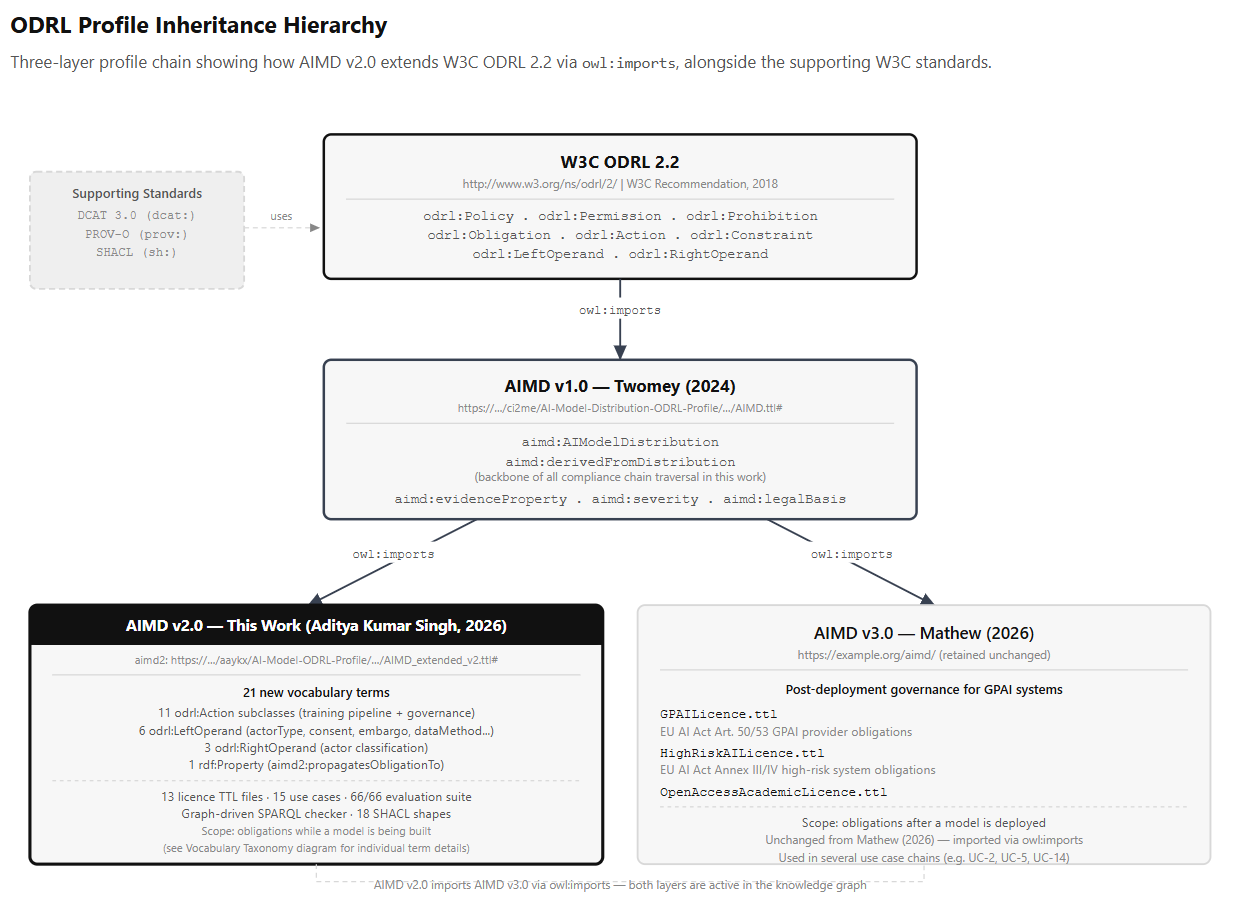
\includegraphics[width=0.95\textwidth]{fig_profile_hierarchy.png}
  \caption[ODRL Profile Inheritance Hierarchy]{%
    The three-layer ODRL profile inheritance chain. W3C ODRL~2.2~\cite{odrl22} (top) provides the foundational rights expression vocabulary. AIMD~v1.0~\cite{twomey2024} (middle) adds AI model distribution metadata terms, most critically \texttt{aimd:derivedFromDistribution}, the property traversed by every compliance checker function. AIMD~v2.0 (this work, bottom left) and AIMD~v3.0~\cite{mathew2026} (bottom right) both extend v1.0 via \texttt{owl:imports}: v2.0 adds 21 new terms targeting training-pipeline obligations; v3.0 adds post-deployment GPAI governance. DCAT~\cite{dcat3}, PROV-O~\cite{provo}, and SHACL~\cite{shacl} are used throughout all layers but do not participate in the inheritance chain.}
  \label{fig:hierarchy}
\end{figure}

\subsection{Reused Standards}

\subsubsection{W3C ODRL 2.2: Open Digital Rights Language}

\textbf{Namespace:} \texttt{http://www.w3.org/ns/odrl/2/}

ODRL~\cite{odrl22} is the W3C Recommendation for expressing rights, permissions, prohibitions, and obligations over digital assets in machine-readable form. It is the primary language of this profile. ODRL's core vocabulary provides:

\begin{description}[leftmargin=2cm, style=nextline]
  \item[\texttt{odrl:Policy}] The root class. Every licence file is an instance of \texttt{odrl:Policy} (and typically also \texttt{odrl:Set}).
  \item[\texttt{odrl:PolicySet}] Groups multiple policies that must be satisfied simultaneously (used in UC-11 for RAG multi-asset governance).
  \item[\texttt{odrl:permission}] A rule granting the right to perform an action, possibly conditional on constraints and duties.
  \item[\texttt{odrl:prohibition}] A rule forbidding an action, possibly conditional on constraints.
  \item[\texttt{odrl:obligation}] An action that must be performed regardless of whether the main activity is permitted.
  \item[\texttt{odrl:duty}] A condition attached to a permission: must be satisfied for the permission to remain valid.
  \item[\texttt{odrl:constraint}] A conditional expression over a left operand, operator, and right operand that gates a rule.
  \item[\texttt{odrl:Action}] The class of all actions that can be governed (e.g.\ \texttt{odrl:distribute}). This profile adds 11 AI-specific subclasses.
  \item[\texttt{odrl:LeftOperand}] Properties of the context that can be tested in constraints (e.g.\ \texttt{odrl:dateTime}, \texttt{odrl:count}). This profile adds 6 new instances.
  \item[\texttt{odrl:RightOperand}] Reference values for constraints (e.g.\ \texttt{CommercialPurpose}). This profile adds 3 new instances.
\end{description}

ODRL was chosen over alternatives (DALICC~\cite{dalicc}, SPDX, Creative Commons REL) because it is a W3C standard, extensible by profiles, and has an active W3C AI Vocabulary Working Group drafting AI-specific extensions. The profile approach means this work can be aligned with that vocabulary as it matures.

\subsubsection{W3C DCAT 3.0: Data Catalog Vocabulary}

\textbf{Namespace:} \texttt{http://www.w3.org/ns/dcat\#}

DCAT~\cite{dcat3} is the W3C Recommendation for describing datasets and data distributions in a machine-readable catalog. In this profile, every AI model, dataset, and training artefact is represented as a \texttt{dcat:Distribution} node. This enables:

\begin{itemize}[noitemsep]
  \item Consistent identification of every artefact in the supply chain via a URI
  \item Linking distributions to their ODRL policies via \texttt{odrl:hasPolicy}
  \item Grouping all 15 use case terminal distributions in a \texttt{dcat:Catalog} for the knowledge graph
  \item Interoperability with existing open data infrastructure (CKAN, data.gov, institutional repositories like TCD TARA)
\end{itemize}

Key DCAT terms used: \texttt{dcat:Distribution}, \texttt{dcat:Catalog}, \texttt{dcat:accessURL}, \texttt{dcat:dataset}.

\subsubsection{W3C PROV-O: Provenance Ontology}

\textbf{Namespace:} \texttt{http://www.w3.org/ns/prov\#}

PROV-O~\cite{provo} is the W3C Recommendation for recording the provenance of data: who created it, from what, and when. In this profile, PROV-O triples are added to every distribution in the knowledge graph to record the training chain as a provenance graph:

\begin{lstlisting}
dcat:OpenResearchLLMDist1
    prov:wasGeneratedBy [
        a prov:Activity ;
        prov:used dcat:CCBYCorpusDist1
    ] .
\end{lstlisting}

This enables provenance-aware compliance: the SHACL multi-hop shape  \linebreak (\texttt{aimd2:MultiHopProvenanceShape}) can detect derivation chains that are more than 3 hops deep and flag them for enhanced scrutiny. PROV-O also provides the audit trail needed for EU AI Act Art.\ 53 training data disclosure.

\subsubsection{Dublin Core Terms (DCT)}

\textbf{Namespace:} \texttt{http://purl.org/dc/terms/}

Dublin Core metadata terms are used throughout for standard bibliographic metadata: \texttt{dct:title}, \texttt{dct:description}, \texttt{dct:created}, \texttt{dct:license}, \texttt{dct:issued}. Crucially, \texttt{dct:license} is used on every distribution node to carry the governing licence URI: this is the primary lookup path used by the SPARQL compliance checker.

\subsubsection{W3C SHACL: Shapes Constraint Language}

\textbf{Namespace:} \texttt{http://www.w3.org/ns/shacl\#}

SHACL~\cite{shacl} is the W3C Recommendation for expressing structural and semantic constraints on RDF graphs. In this project, SHACL serves as a static validation layer on top of the dynamic SPARQL-based checker. The file \texttt{AIMD\_v2\_shapes.ttl} defines 18 shapes:

\begin{itemize}[noitemsep]
  \item 7 \emph{property-path shapes} (\texttt{sh:NodeShape} with \texttt{sh:property}) enforcing structural requirements on \texttt{dcat:Distribution} nodes
  \item 11 \emph{SPARQL constraint shapes} (\texttt{sh:SPARQLConstraint}) encoding the same logic as the JavaScript checker functions, enabling offline batch validation
\end{itemize}

SHACL operates at graph-import time (validating the knowledge graph when loaded into GraphDB), while the JavaScript checker operates at query time (validating specific distributions on demand).

\subsubsection{OWL, RDF, RDFS, XSD}

Standard W3C semantic web foundations:
\begin{itemize}[noitemsep]
  \item \textbf{RDF} (\texttt{rdf:}): the triple data model; \texttt{rdf:Property} used for  \linebreak\texttt{aimd2:propagatesObligationTo}
  \item \textbf{RDFS} (\texttt{rdfs:}): \texttt{rdfs:label}, \texttt{rdfs:comment}, \texttt{rdfs:domain}, \texttt{rdfs:range}, \texttt{rdfs:isDefinedBy}
  \item \textbf{OWL} (\texttt{owl:}): \texttt{owl:Ontology}, \texttt{owl:imports}, \texttt{owl:versionInfo}
  \item \textbf{XSD} (\texttt{xsd:}): typed literals: \texttt{xsd:date}, \texttt{xsd:integer}, \texttt{xsd:string}
\end{itemize}

\subsubsection{SKOS: Simple Knowledge Organization System}

\textbf{Namespace:} \texttt{http://www.w3.org/2004/02/skos/core\#}

Used in \texttt{AIMD\_extended\_v2.ttl} to group all 21 new vocabulary terms into a \texttt{skos:Collection} with a \texttt{skos:prefLabel} and \texttt{skos:scopeNote}. This makes the vocabulary machine-discoverable as a thesaurus entry without needing to enumerate terms from OWL alone.

\subsection{Inherited AI Model Distribution Profiles}

\subsubsection{AIMD v1.0: Twomey (2024)}

\textbf{Namespace:} \texttt{https://raw.githubusercontent.com/ci2me/AI-Model-\linebreak Distribution-ODRL-Profile/main /AIMD.ttl\#}

Cian Twomey's original profile~\cite{twomey2024} established the infrastructure for ODRL-based AI model distribution governance. Key terms inherited and used throughout this project:

\begin{itemize}[noitemsep]
  \item \texttt{aimd:AIModelDistribution}: the RDF class typing all distribution nodes in the knowledge graph
  \item \texttt{aimd:derivedFromDistribution}: the core provenance property linking derived distributions to their sources (the backbone of all multi-hop chain traversal)
  \item \texttt{aimd:evidenceProperty}, \texttt{aimd:severity}, \texttt{aimd:legalBasis}, \texttt{aimd:checkDescription}: annotation properties used on every new action term in v2.0
\end{itemize}

The \texttt{aimd:derivedFromDistribution} property is the most critical inherited term: every compliance checker function traverses it to walk up (or down) the training chain.

\subsubsection{AIMD v3.0: Mathew (2026)}

\textbf{Namespace:} \texttt{https://example.org/aimd/} (retained unchanged in \texttt{AIMD\_extended.ttl})

Diya Mathew's profile~\cite{mathew2026} extended Twomey's work with distribution-level governance for deployed AI models, including:

\begin{itemize}[noitemsep]
  \item \texttt{GPAILicence.ttl}: GPAI provider compliance (EU AI Act Art.\ 50/53)
  \item \texttt{HighRiskAILicence.ttl}: EU AI Act Annex III/IV high-risk system obligations
  \item \texttt{OpenAccessAcademicLicence.ttl}: open academic access governance
\end{itemize}

These files are imported by \texttt{AIMD\_extended\_v2.ttl} via \texttt{owl:imports} and are used in several use cases (e.g.\ UC-2 reuses \texttt{GPAILicence.ttl} as the commercial product's downstream policy). Crucially, none of Diya's files were modified. The distinction between the two works is:

\begin{itemize}[noitemsep]
  \item \textbf{Mathew (v3.0)}: governs AI model \emph{distribution after it is built}
  \item \textbf{This work (v2.0)}: governs the legal obligations that arise \emph{while it is being built}
\end{itemize}

\newpage

% ─────────────────────────────────────────────────────────────────────────────
\section{AIMD Extended Profile v2.0: New Vocabulary}
% ─────────────────────────────────────────────────────────────────────────────

The profile is defined in \texttt{AIMD\_extended\_v2.ttl}. It declares 21 new ODRL vocabulary terms at the namespace \texttt{https://raw.githubusercontent.com/aaykx/AI-Model-ODRL-Profile/main/AIMD_extended_v2.ttl#}, structured as an \texttt{owl:Ontology} that is simultaneously an ODRL \texttt{profile:Profile}.

\subsection{Eleven New Action Terms}

Each action term is an instance of \texttt{odrl:Action} and carries four annotation properties:

\begin{itemize}[noitemsep]
  \item \texttt{aimd:evidenceProperty}: the data property on a \texttt{dcat:Distribution} that constitutes evidence the action was performed
  \item \texttt{aimd:severity}: \texttt{"mandatory"} or \texttt{"recommended"}
  \item \texttt{aimd:legalBasis}: the regulation(s) motivating the obligation
  \item \texttt{aimd:checkDescription}: what the SPARQL checker tests for
\end{itemize}

\begin{longtable}{@{}>{\footnotesize}p{6.0cm}>{\footnotesize}p{4.5cm}>{\footnotesize}p{4.3cm}@{}}
\toprule
\textbf{Term} & \textbf{Evidence Property} & \textbf{Legal Basis / Purpose} \\
\midrule
\endhead
\texttt{aimd2:AITraining} & \texttt{trainingDatasetURL} & DSM Directive Arts.\ 3/4; OSAID 1.0. Declares the dataset used for pre-training. \\[4pt]
\texttt{aimd2:FineTuning} & \texttt{baseModelURL} & OSAID 1.0; EU AI Act Art.\ 53. Declares the base model a fine-tuned model derives from. \\[4pt]
\texttt{aimd2:RAGIngestion} & \texttt{ragCorpusPolicy} & Novel operational term. Declares the policy governing the document corpus indexed for RAG. \\[4pt]
\texttt{aimd2:RLHFTraining} & \texttt{rlhfDataPolicy} & GDPR Arts.\ 13/14; EU AI Act Art.\ 10. Declares the human feedback data governance policy. \\[4pt]
\texttt{aimd2:AIInference} & \texttt{inferenceEndpointURL} & Novel operational term. Identifies the deployed inference endpoint. \\[4pt]
\texttt{aimd2:ModelSharing} & \texttt{modelWeightsURL} & OSAID 1.0 Share freedom. Requires public publication of model weights. \\[4pt]
\texttt{aimd2:InheritSourceLicence} & \texttt{downstreamLicenceURI} & CC-BY-SA ShareAlike; GPL copyleft. Requires the downstream distribution to carry the source's licence. \\[4pt]
\texttt{aimd2:InheritSourceProhibitions} & \texttt{derivedModelLicenceURI} & RAIL licence; EU AI Act Annex V; Proprietary ToS. Requires prohibited uses to survive into derived models. \\[4pt]
\texttt{aimd2:DeclareRLHFDataUse} & \texttt{rlhfDisclosureURL} & GDPR Art.\ 13; EU AI Act Art.\ 10. Requires a public transparency notice for RLHF data collection. \\[4pt]
\texttt{aimd2:ReportSecurityIncidents} & \texttt{securityContactURL} & G7 SBOM Cluster 6; EU AI Act Art.\ 72. Requires a published security contact. \\[4pt]
\texttt{aimd2:ComplyWithArticle50} & \texttt{article50PolicyURL} & EU AI Act Art.\ 50. Requires a published policy for AI-generated content disclosure and labelling. \\
\bottomrule
\caption{New ODRL Action terms in AIMD v2.0}
\end{longtable}

\subsection{Nine New Operand Terms}

\textbf{Right Operands} (values used in constraint right-hand sides):

\begin{itemize}[noitemsep]
  \item \texttt{aimd2:CommercialPurpose}: identifies commercial actors, who are excluded from the DSM Art.\ 3 research TDM exception
  \item \texttt{aimd2:ScientificResearchPurpose}: identifies actors qualifying for the DSM Art.\ 3 research exception
  \item \texttt{aimd2:RecognisedResearchOrganisation}: constrains the Art.\ 3 exception to qualifying institutions (universities, research centres)
\end{itemize}

\textbf{Left Operands} (constraint axes testable in SPARQL):

\begin{itemize}[noitemsep]
  \item \texttt{aimd2:EmbargoEndDate}: the date after which embargoed content may be accessed; evaluated against SPARQL \texttt{NOW()}
  \item \texttt{aimd2:userConsentStatus}: GDPR consent status for RLHF data; values include \texttt{"given"}, \texttt{"withdrawn"}, \texttt{"not-required"}
  \item \texttt{aimd2:downstreamLicence}: the licence URI of the derivative, checked for copyleft compatibility
  \item \texttt{aimd2:actorType}: discriminates commercial from research actors; values \texttt{"commercial"}, \texttt{"research"}, \texttt{"competitor"}
  \item \texttt{aimd2:dataGenerationMethod}: discriminates synthetic from real data; values \texttt{"synthetic"}, \texttt{"real"}, \texttt{"mixed"}
  \item \texttt{aimd2:deploymentContext}: distinguishes network API deployment from local deployment; triggers AGPL \S 13 provisions
\end{itemize}

\subsection{One New RDF Property}

\texttt{aimd2:propagatesObligationTo} is a plain \texttt{rdf:Property} with domain and range \texttt{odrl:Policy}. It links an upstream ODRL policy to any downstream policy that must inherit its obligations. This property is the machine-readable encoding of multi-hop obligation propagation: analogous to the way a software supply chain must carry GPL notices through every layer.

Every licence TTL file declares this property on itself, typically as a self-referential link (the policy propagates to itself and all downstream policies that govern derivative distributions).

\begin{figure}[htbp]
  \centering
  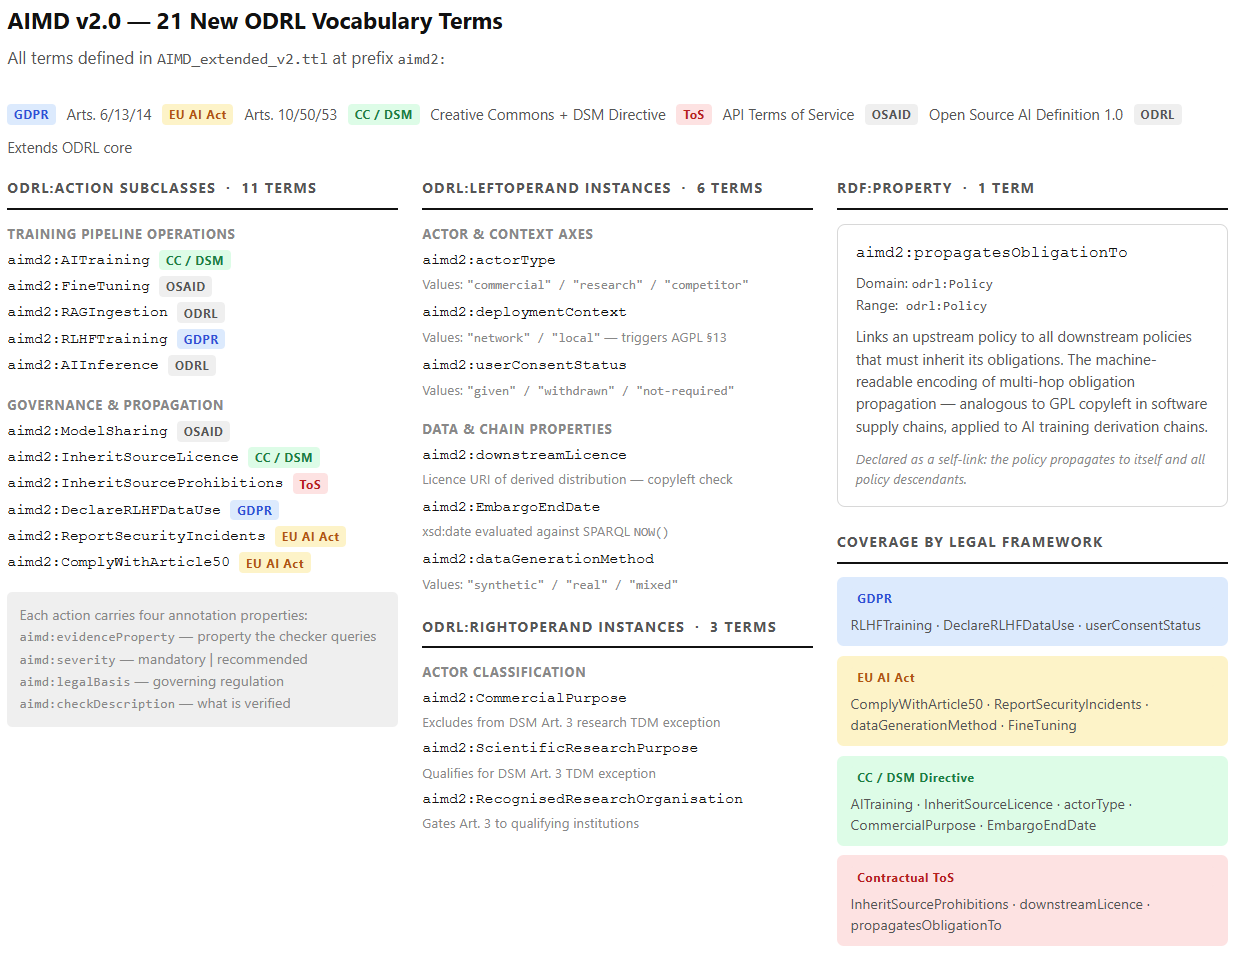
\includegraphics[width=0.95\textwidth]{fig_vocab_taxonomy.png}
  \caption[AIMD v2.0 Vocabulary Taxonomy]{%
    Taxonomy of the 21 new ODRL vocabulary terms defined in \texttt{AIMD\_extended\_v2.ttl}. \emph{Left:} 11 new \texttt{odrl:Action} subclasses, split between training pipeline operations (\texttt{AITraining}, \texttt{FineTuning}, \texttt{RAGIngestion}, \texttt{RLHFTraining}, \texttt{AIInference}) and governance actions (\texttt{ModelSharing}, \texttt{InheritSourceLicence}, \texttt{InheritSourceProhibitions}, \texttt{DeclareRLHFDataUse}, \texttt{ReportSecurityIncidents}, \texttt{ComplyWithArticle50}). Each action carries four annotation properties---\texttt{evidenceProperty}, \texttt{severity}, \texttt{legalBasis}, \texttt{checkDescription}---consumed by the SPARQL checker at query time. \emph{Centre:} 6 \texttt{odrl:LeftOperand} and 3 \texttt{odrl:RightOperand} instances defining the constraint axes used across all use cases. \emph{Right:} The \texttt{aimd2:propagatesObligationTo} property and a summary of coverage by legal framework (GDPR, EU AI Act, CC/DSM, Contractual ToS).}
  \label{fig:vocab}
\end{figure}

\newpage

% ─────────────────────────────────────────────────────────────────────────────
\section{System Architecture: Files Added}
% ─────────────────────────────────────────────────────────────────────────────

\subsection{AIMD\_extended\_v2.ttl: The Vocabulary File}

This is the authoritative ODRL profile declaration. It declares the \texttt{aimd2:} ontology as both an \texttt{owl:Ontology} and a \texttt{profile:Profile}~\cite{profilesvocab} (W3C Profiles Vocabulary). It contains:

\begin{itemize}[noitemsep]
  \item The 21 new vocabulary terms described in Section~3
  \item \texttt{owl:imports} links to both AIMD v1.0 and AIMD v3.0 (Diya's work)
  \item A \texttt{skos:Collection} grouping all 21 terms for machine-discoverability
  \item A \texttt{profile:isProfileOf <http://www.w3.org/ns/odrl/2/>} declaration asserting this is an ODRL sub-profile
\end{itemize}

This file must be loaded into GraphDB before any licence or knowledge graph file.

\subsection{13 Licence TTL Files}

Each licence TTL file is a standalone ODRL policy document encoding the rights, duties, prohibitions, and obligations of a specific licence type as it applies to AI model training. The files are described individually in Section~5. Common structural features:

\begin{lstlisting}
<https://example.com/policy/ExampleLicence>
    a odrl:Policy, odrl:Set ;
    dct:title "..." ;
    dct:description "..." ;
    dct:created "2026-06-30"^^xsd:date ;

    odrl:permission [ odrl:action aimd2:AITraining ; ... ] ;
    odrl:prohibition [ odrl:action aimd2:AITraining ; ... ] ;
    odrl:obligation [ odrl:action aimd2:ComplyWithArticle50 ] ;

    aimd2:propagatesObligationTo <https://example.com/policy/ExampleLicence> .
\end{lstlisting}

\subsection{AIMD\_v2\_knowledge\_graph.ttl: The Test Data Seed}

This file contains all 15 use case distribution chains as importable Turtle triples, enabling GraphDB to be seeded by file import rather than running the Node.js server. It contains:

\begin{itemize}[noitemsep]
  \item A \texttt{dcat:Catalog} at \texttt{<https://raw.githubusercontent.com/aaykx/AI-Model-ODRL-Profile/main/AIMD_v2_knowledge_graph.ttl>} listing all 15 terminal distributions
  \item All intermediate distribution nodes in every chain (approximately 40 distribution nodes total)
  \item \texttt{dcat:accessURL}, \texttt{dct:license}, \texttt{odrl:hasPolicy}, and all signal properties (\texttt{aimd2:actorType}, \texttt{aimd2:trainingDatasetURL}, etc.)
  \item \texttt{aimd:derivedFromDistribution} edges forming the chain graph
  \item \texttt{prov:wasGeneratedBy} blank nodes on every distribution for PROV-O provenance
  \item \texttt{aimd2:propagatesObligationTo} links on each chain's anchor policy
\end{itemize}

This file serves two purposes: it is the test fixture for the compliance checker, and it is the reference implementation showing how AIMD v2.0 distributions should be represented in practice.

\subsection{server\_v2.js: The Graph-Driven Compliance Checker}

The compliance checker is a Node.js server (built on the Express framework) that connects to a local GraphDB Free v10.x SPARQL endpoint. It is structured in seven phases:

\begin{description}[leftmargin=3cm, style=nextline]
  \item[Phase 1] Server startup and GraphDB connection verification
  \item[Phase 2] Named graph creation (isolates test data from production data)
  \item[Phase 3] SPARQL \texttt{INSERT DATA} seeding of all 15 use case chains
  \item[Phase 4] AIMD v2.0 vocabulary annotation loading
  \item[Phase 5] Query verification (basic sanity checks)
  \item[Phase 6] Per-use-case compliance checks (12 checker functions)
  \item[Phase 7] Smoke test suite (23 automated assertions, \texttt{npm test})
\end{description}

\textbf{Graph-driven design:} The checker is not hardcoded to specific licence names. Instead, it queries the RDF graph for ODRL obligation patterns and tests whether the distribution carries the evidence property declared on each action term. Adding a new obligation only requires adding the ODRL triple to the licence file: no code change is needed.

\begin{figure}[htbp]
  \centering
  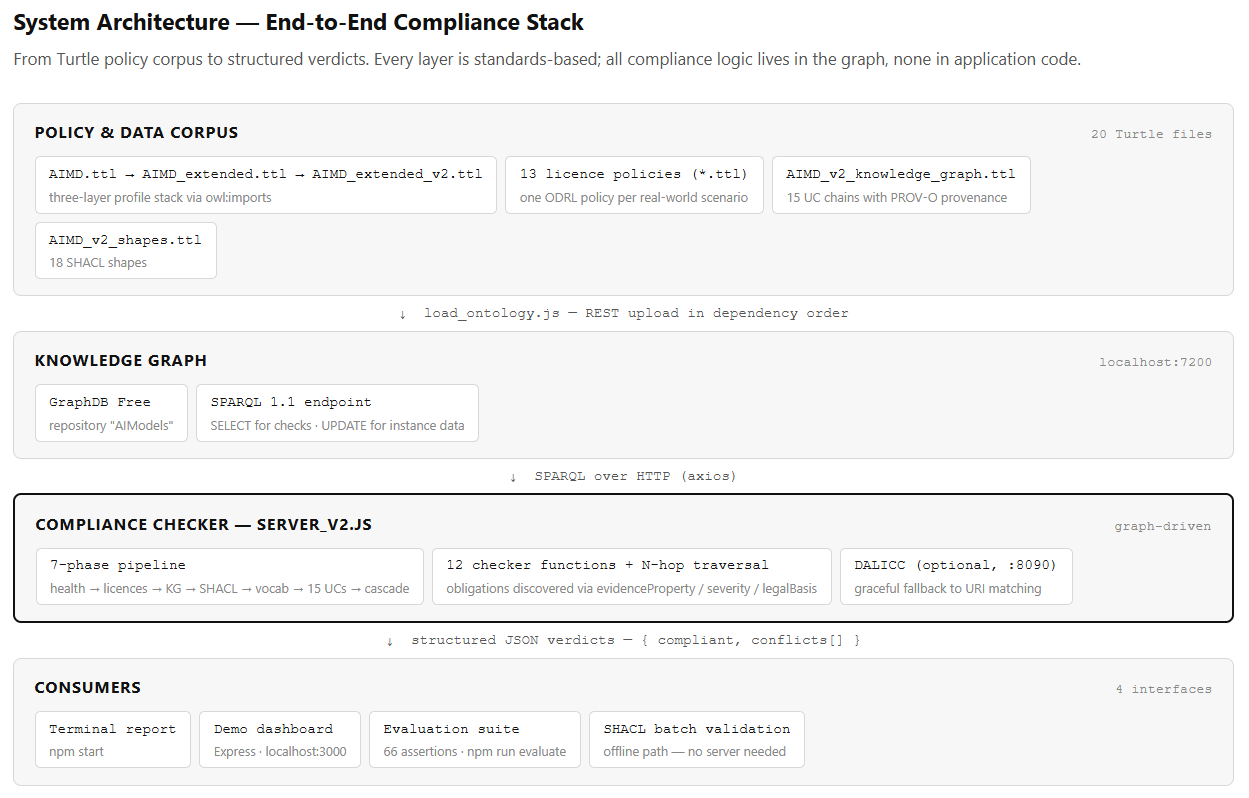
\includegraphics[width=0.9\textwidth]{fig_architecture.png}
  \caption[System Architecture]{%
    End-to-end architecture of the AIMD~v2.0 compliance stack. The policy and data corpus (20 Turtle files: the three-layer profile stack composed via \texttt{owl:imports}, 13 licence policies, the use-case knowledge graph, and 18 SHACL shapes) is loaded into a GraphDB repository by \texttt{load\_ontology.js} in dependency order. The compliance checker (\texttt{server\_v2.js}) queries the SPARQL~1.1 endpoint over HTTP and executes a seven-phase pipeline; obligations are discovered from the graph via the \texttt{aimd:evidenceProperty}, \texttt{aimd:severity} and \texttt{aimd:legalBasis} annotations rather than being hardcoded. Structured JSON verdicts are consumed by four interfaces: the terminal report, the demonstration dashboard, the 66-assertion evaluation suite, and offline SHACL batch validation. DALICC integration is optional, with graceful fallback to URI matching~\cite{dalicc}.}
  \label{fig:architecture}
\end{figure}

\textbf{Multi-hop traversal:} The \texttt{checkNHopChain()} function \linebreak traverses \texttt{aimd:derivedFromDistribution} iteratively (not via SPARQL property paths) to safely handle cycles and enforce a configurable \texttt{maxHops} limit.

\textbf{Checker functions:}

\begin{enumerate}[noitemsep]
  \item \texttt{checkCommercialConflict()}: NC licence vs commercial actor (UC-2, UC-5)
  \item \texttt{checkCopyleftPropagation()}: ShareAlike obligation stripping (UC-3, UC-5)
  \item \texttt{checkEmbargoCompliance()}: temporal embargo gate using SPARQL \texttt{NOW()} (UC-4)
  \item \texttt{checkMultiSourceConflict()}: multi-parent licence conflict aggregation (UC-5)
  \item \texttt{checkDistillationProhibition()}: proprietary ToS + Layer 2 constraint inheritance (UC-6, UC-15)
  \item \texttt{checkNHopChain()}: generic N-hop chain with obligation inheritance (UC-1, UC-7, UC-13, UC-14)
  \item \texttt{checkAGPLNetworkTrigger()}: AGPL \S 13 network copyleft (UC-8, UC-15)
  \item \texttt{checkRLHFConsent()}: GDPR consent verification (UC-9, UC-15)
  \item \texttt{checkSyntheticDataDisclosure()}: EU AI Act Art.\ 53 synthetic data gap (UC-10, UC-15)
  \item \texttt{checkRAGPolicySet()}: multi-asset PolicySet composition (UC-11)
  \item \texttt{checkMoEInheritance()}: Mixture-of-Experts licence inheritance (UC-12, UC-15)
  \item \texttt{checkCascadingConflicts()}: UC-15 all-conflict aggregation without short-circuit
\end{enumerate}

\begin{figure}[htbp]
  \centering
  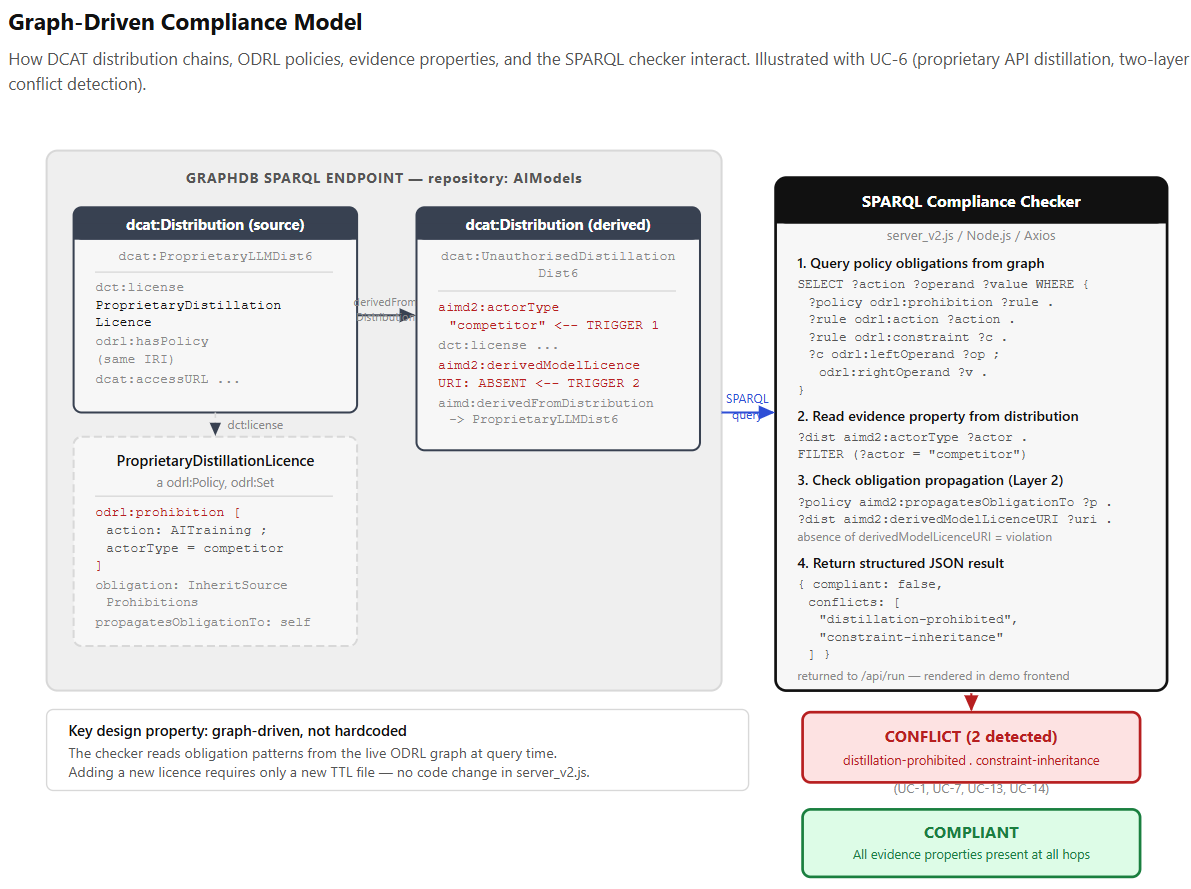
\includegraphics[width=0.95\textwidth]{fig_compliance_model.png}
  \caption[Graph-Driven Compliance Model]{%
    The graph-driven compliance model, illustrated with UC-6 (proprietary API distillation). A source \texttt{dcat:Distribution} node (\texttt{ProprietaryLLMDist6}) carries a \texttt{dct:license} link to its governing ODRL policy (\texttt{ProprietaryDistillationLicence}), which encodes a prohibition against AI Training by competitor actors and an \texttt{InheritSourceProhibitions} obligation. The derived distribution (\texttt{UnauthorisedDistillationDist6}) carries \texttt{aimd2:actorType~=~"competitor"} (Layer~1 trigger) and is missing \texttt{aimd2:derivedModelLicenceURI} (Layer~2 trigger). The SPARQL compliance checker (\texttt{server\_v2.js}) operates in four steps: (1)~query policy obligations from the live RDF graph; (2)~match evidence properties on the distribution node; (3)~verify propagated obligations via \texttt{aimd2:propagatesObligationTo}; (4)~return a structured JSON result accumulating all detected conflicts. Crucially, the checker is \emph{graph-driven}: no obligation pattern is hardcoded in JavaScript; adding a new licence type requires only a new TTL file.}
  \label{fig:compliance}
\end{figure}

\subsection{AIMD\_v2\_shapes.ttl: The SHACL Validation Suite}

Defines 18 SHACL shapes mirroring the checker functions, enabling offline batch validation:

\textbf{7 Property-Path Shapes} (structural requirements):

\begin{itemize}[noitemsep]
  \item \texttt{aimd2:AIModelDistributionShape}: all \texttt{dcat:Distribution} nodes require \texttt{dct:license}, \texttt{dcat:accessURL}, \texttt{dct:issued}, \texttt{odrl:hasPolicy}
  \item \texttt{aimd2:TrainingDistributionShape}: distributions with \texttt{trainingDatasetURL} must also carry \texttt{modelWeightsURL}, \texttt{article50PolicyURL}, \texttt{downstreamLicenceURI}
  \item \texttt{aimd2:FineTuningDistributionShape}, \texttt{aimd2:RLHFDistributionShape}, \texttt{aimd2:RAGDistributionShape}, \texttt{aimd2:SyntheticDataDistributionShape}, \texttt{aimd2:GPAIComplianceShape}
\end{itemize}

\textbf{11 SPARQL Constraint Shapes} (semantic compliance checks):

\begin{itemize}[noitemsep]
  \item \texttt{aimd2:NCConflictShape} (UC-2, UC-5)
  \item \texttt{aimd2:CopyleftPropagationShape} (UC-3)
  \item \texttt{aimd2:EmbargoConstraintShape} (UC-4)
  \item \texttt{aimd2:DistillationProhibitionShape} (UC-6, UC-15)
  \item \texttt{aimd2:AGPLNetworkTriggerShape} (UC-8, UC-15)
  \item \texttt{aimd2:RLHFConsentCrossCheckShape} (UC-9)
  \item \texttt{aimd2:SyntheticDataDisclosureGapShape} (UC-10, UC-15)
  \item \texttt{aimd2:RAGPolicySetShape} (UC-11)
  \item \texttt{aimd2:MoEObligationInheritanceShape} (UC-12, UC-15)
  \item \texttt{aimd2:MultiHopProvenanceShape} (UC-14)
  \item \texttt{aimd2:CascadingConflictShape} (UC-15)
\end{itemize}

\newpage

% ─────────────────────────────────────────────────────────────────────────────
\section{Use Cases and Licence Files}
% ─────────────────────────────────────────────────────────────────────────────

Each use case represents a real-world scenario drawn from current AI development practice. The table below summarises all 15 use cases; detailed explanations follow.

\begin{longtable}{@{}p{0.7cm}p{5.0cm}p{2.0cm}p{6.0cm}@{}}
\toprule
\textbf{UC} & \textbf{Chain} & \textbf{Result} & \textbf{Legal Trigger} \\
\midrule
\endhead
1 & CC-BY Corpus $\rightarrow$ Open Research LLM & \compliant & DSM Art.\ 3 research TDM \\
2 & CC-BY-NC Dataset $\rightarrow$ Commercial Product & \violated{CONFLICT} & NC prohibition vs commercial actor \\
3 & CC-BY-SA Corpus $\rightarrow$ Fine-Tuned Model & \violated{VIOLATION} & ShareAlike obligation stripped \\
4 & Embargoed Preprint $\rightarrow$ Premature RAG & \violated{EMBARGO} & DSM Art.\ 3(1) lawful access \\
5 & Multi-source (CC-BY + NC + SA) $\rightarrow$ GPAI & \violated{CONFLICT} & Simultaneous multi-source conflicts \\
6 & Proprietary LLM API $\rightarrow$ Distillation & \violated{PROHIBITED} & ToS competitor prohibition \\
7 & Apache 2.0 Base $\rightarrow$ MIT Fine-Tune & \compliant & Permissive-to-permissive baseline \\
8 & Apache $\rightarrow$ AGPL $\rightarrow$ Network API & \violated{VIOLATION} & AGPLv3 \S 13 network copyleft \\
9 & Open Model $\rightarrow$ RLHF $\rightarrow$ Aligned & \violated{VIOLATION} & GDPR Art.\ 6 consent absent \\
10 & Proprietary Teacher $\rightarrow$ Synthetic $\rightarrow$ Open & \violated{GAP} & EU AI Act Art.\ 53(1)(c) \\
11 & Retriever + Corpus $\rightarrow$ RAG Generator & \policyset & IDS-RAM 4.0 multi-asset PolicySet \\
12 & Expert A + Expert B (Llama) + C $\rightarrow$ MoE & \violated{FAILURE} & Llama MAU threshold not inherited \\
13 & Planner LLM $\rightarrow$ Executor LLM & \compliant & Inference-only true negative \\
14 & CC-BY $\rightarrow$ Distil $\rightarrow$ SLM $\rightarrow$ GPAI API & \compliant & 3-hop attribution chain preserved \\
15 & Prop.\ Data $\rightarrow$ Closed $\rightarrow$ Distil $\rightarrow$ MoE $\rightarrow$ Product & \violated{CASCADING} & 3 simultaneous unresolvable conflicts \\
\bottomrule
\caption{Summary of all 15 use cases}
\end{longtable}

\begin{figure}[htbp]
  \centering
  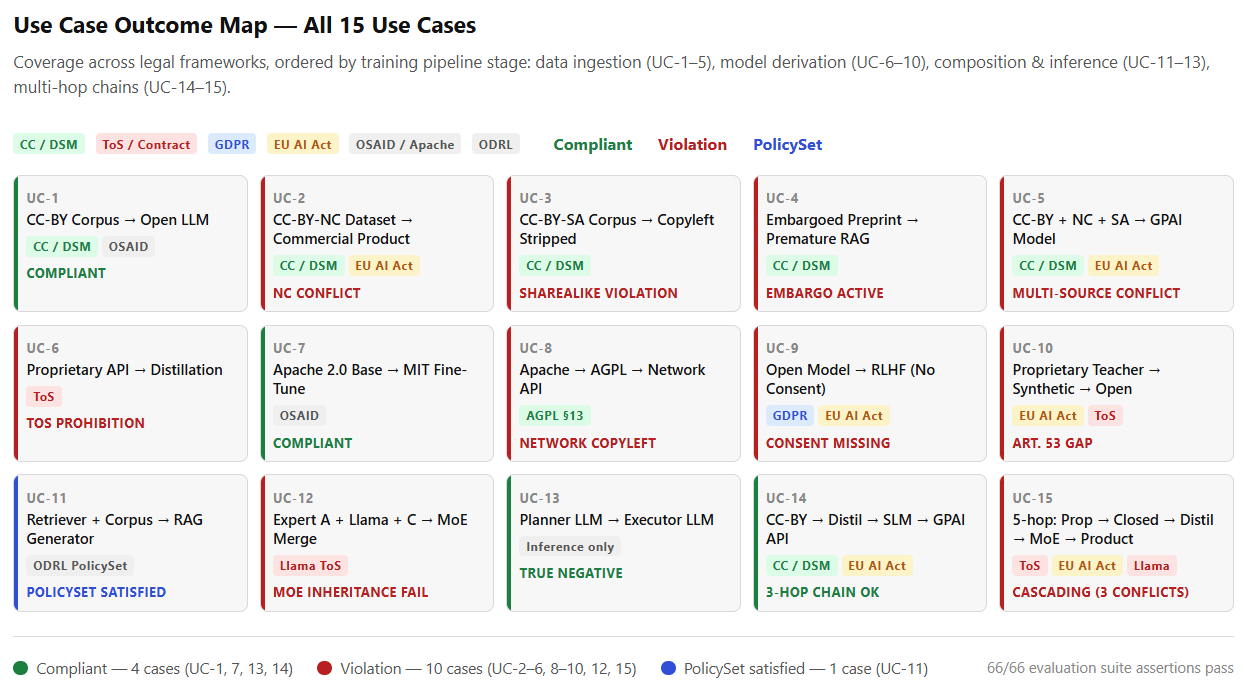
\includegraphics[width=0.95\textwidth]{fig_usecase_map.png}
  \caption[Use Case Outcome Map]{%
    Overview of all 15 use cases evaluated by the AIMD~v2.0 compliance checker, ordered by training pipeline stage: data ingestion (UC-1--5), model derivation (UC-6--10), composition and inference (UC-11--13), and multi-hop chains (UC-14--15). Left border colour indicates verdict: green (compliant), red (violation), blue (PolicySet). Of the 15 cases, 4 are compliant (UC-1, 7, 13, 14), 10 are violations spanning Creative Commons restrictions, AGPL copyleft, GDPR consent gaps, EU AI Act Art.\ 53 disclosure requirements, and proprietary ToS prohibitions, and 1 satisfies a multi-asset PolicySet (UC-11). UC-13 is a true-negative anti-regression test confirming the checker does not apply training-pipeline obligations to inference-only chains. UC-15 is the stress test, accumulating three simultaneous unresolvable conflicts across a 5-hop chain (verified by assertion E-23: \texttt{conflicts.length~$\geq$~3}). All 15 verdicts are verified by the 66-assertion evaluation suite.}
  \label{fig:ucmap}
\end{figure}

% ──────────────────────────────────────────────────────────────────────────────
\subsection{UC-1: CC-BY Academic Corpus to Open Research LLM}
\textbf{Licence file:} \texttt{OpenResearchLLMLicence.ttl}\\[2pt]
\textbf{Result:} \compliant\\[4pt]
\textbf{Legal basis:} CC-BY 4.0~\cite{ccby40} \S 3(a); DSM Directive~\cite{dsm2019} Art.\ 3(1); OSAID 1.0~\cite{osaid10}

\textbf{Chain:} \texttt{CCBYCorpusDist1} $\rightarrow$ \texttt{OpenResearchLLMDist1}

This is the \emph{baseline compliant case}: the clean scenario that every other use case is measured against. A university research lab downloads a CC-BY-licensed corpus from TCD TARA, trains an open LLM, and publishes the model with all metadata intact.

\textbf{The licence models:}
\begin{itemize}[noitemsep]
  \item \emph{Permission:} AI Training is permitted for actors identified as \linebreak\texttt{RecognisedResearchOrganisation} (DSM Art.\ 3 TDM exception), with three duties: \texttt{ModelSharing}, \texttt{InheritSourceLicence}, \texttt{ComplyWithArticle50}
  \item \emph{Prohibition:} AI Training by \texttt{CommercialPurpose} actors is prohibited (Art.\ 4(3) opt-out)
  \item \emph{Propagation:} Attribution obligation flows to all downstream policies
\end{itemize}

\textbf{Checker logic:} Verifies \texttt{trainingDatasetURL}, \texttt{modelWeightsURL}, \texttt{downstreamLicenceURI}, and \texttt{article50PolicyURL} are all present. All four are present in \texttt{OpenResearchLLMDist1} $\Rightarrow$ \compliant.

This case also serves as the licence for all hops in UC-14 (the 3-hop GPAI chain), demonstrating that the same licence file can appear at multiple points in a chain.

% ──────────────────────────────────────────────────────────────────────────────
\subsection{UC-2: CC-BY-NC Dataset to Commercial AI Product}
\textbf{Licence file:} \texttt{CommercialConflictLicence.ttl}\\[2pt]
\textbf{Result:} \violated{NC CONFLICT}\\[4pt]
\textbf{Legal basis:} CC-BY-NC 4.0~\cite{ccbync40} \S 3(b); DSM Directive~\cite{dsm2019} Art.\ 4(3); EU AI Act~\cite{euaiact2024} Art.\ 53(1)(c)

\textbf{Chain:} \texttt{CCBYNCDatasetDist2} $\rightarrow$ \texttt{CommercialProductDist2}

CC-BY-NC is one of the most common dataset licences in AI research. The NC clause prohibits commercial use. When a company trains a commercial AI product on such a dataset, there is a direct legal conflict that existing tools fail to detect.

\textbf{The licence models:}
\begin{itemize}[noitemsep]
  \item \emph{Permission:} AI Training permitted for non-commercial actors only (\texttt{actorType neq CommercialPurpose})
  \item \emph{Prohibition 1:} AI Training by \texttt{CommercialPurpose} actors: this is the conflict trigger
  \item \emph{Prohibition 2:} Commercial \texttt{ModelSharing}: even redistribution of a commercially trained model is prohibited
  \item \emph{Obligation:} \texttt{InheritSourceProhibitions}: NC restriction propagates downstream
\end{itemize}

\textbf{Legal nuance:} DSM Art.\ 4(3) allows rights holders to machine-readably opt out of the general TDM exception. A CC-BY-NC licence \emph{is} that machine-readable opt-out for commercial actors. EU AI Act Art.\ 53(1)(c) requires GPAI providers to honour this opt-out. This licence file is the machine-readable expression of both.

\textbf{Checker logic:} Detects \texttt{actorType="commercial"} on the derived distribution and a commercial-training prohibition on the parent licence $\Rightarrow$ \violated{CONFLICT}.

% ──────────────────────────────────────────────────────────────────────────────
\subsection{UC-3: CC-BY-SA Corpus to Fine-Tuned Model (Copyleft Stripped)}
\textbf{Licence file:} \texttt{CopyleftPropagationLicence.ttl}\\[2pt]
\textbf{Result:} \violated{COPYLEFT VIOLATION}\\[4pt]
\textbf{Legal basis:} CC-BY-SA 4.0~\cite{ccbysa40} \S 3(b) ShareAlike; \textit{Andersen v.\ Stability AI} (trial September 2026)

\textbf{Chain:} \texttt{CCBYSACorpusDist3} $\rightarrow$ \texttt{CopyleftViolatingModelDist3}

CC-BY-SA is a copyleft licence requiring derivatives to be released under the same (or compatible) licence. Jewitt et al.\ (2025) found that 35.5\% of model-to-application licence transitions strip or weaken restrictive clauses like ShareAlike.

\textbf{The licence models:}
\begin{itemize}[noitemsep]
  \item \emph{Permission:} Fine-Tuning permitted only if \texttt{downstreamLicence} is compatible with CC-BY-SA (\texttt{isA CopyleftPropagationLicence}), with duties to carry \texttt{downstreamLicenceURI} and publish weights
  \item \emph{Prohibition:} Model Sharing with an incompatible (or absent) downstream licence URI
\end{itemize}

\textbf{Legal uncertainty:} Whether trained model weights constitute a derivative work of training data is the question \textit{Andersen v.\ Stability AI} (trial September 2026) may answer. The checker does not take a legal position: it detects whether the ShareAlike obligation has been honoured if it exists. If law settles the other way, only the expected result changes.

\textbf{Checker logic:} Detects \texttt{InheritSourceLicence} obligation on the parent policy; checks that \texttt{CopyleftViolatingModelDist3} carries \texttt{downstreamLicenceURI}: absent $\Rightarrow$ \violated{VIOLATION}.

% ──────────────────────────────────────────────────────────────────────────────
\subsection{UC-4: Embargoed Preprint to Premature RAG Ingestion}
\textbf{Licence file:} \texttt{EmbargoedCorpusLicence.ttl}\\[2pt]
\textbf{Result:} \violated{EMBARGO ACTIVE}\\[4pt]
\textbf{Legal basis:} DSM Directive~\cite{dsm2019} Art.\ 3(1) lawful access precondition; TCD TARA embargo policy

\textbf{Chain:} \texttt{EmbargoedPreprintDist4} $\rightarrow$ \texttt{PrematureRAGDist4}

Academic institutions routinely place embargoes on PhD theses and preprints. DSM Art.\ 3(1) requires lawful access as a precondition for the TDM research exception. If the document is under embargo, the exception does not apply.

\textbf{The licence models:}
\begin{itemize}[noitemsep]
  \item \emph{Permission:} RAG Ingestion permitted only when \texttt{dateTime >= EmbargoEndDate} (evaluated at query time via SPARQL \texttt{NOW()})
  \item \emph{Prohibition 1:} RAG Ingestion while \texttt{NOW() < EmbargoEndDate}
  \item \emph{Prohibition 2:} AI Training on embargoed content for the same reason
\end{itemize}

\textbf{Key design decision:} The embargo end date (\texttt{2027-06-30}) is stored in the distribution data, not hardcoded in the licence. The SPARQL checker uses \texttt{FILTER (?embargoEnd > NOW())}: the same triple that produces \violated{EMBARGO} today produces \compliant automatically after the embargo lapses, with no code or data change.

\textbf{Checker logic:} Finds \texttt{EmbargoEndDate = 2027-06-30}; compares against \texttt{NOW()} (2026) $\Rightarrow$ \violated{EMBARGO ACTIVE}.

% ──────────────────────────────────────────────────────────────────────────────
\subsection{UC-5: Multi-Source Corpus (CC-BY + CC-BY-NC + CC-BY-SA) to GPAI Model}
\textbf{Licence files:} \texttt{OpenResearchLLMLicence.ttl}, \texttt{CommercialConflictLicence.ttl}, \texttt{CopyleftPropagationLicence.ttl}\\[2pt]
\textbf{Result:} \violated{MULTI-SOURCE CONFLICT}\\[4pt]
\textbf{Legal basis:} EU AI Act~\cite{euaiact2024} Art.\ 53(1)(c); DALICC~\cite{dalicc} compatibility framework

\textbf{Chain:} \texttt{MultiSourceCCBYDist5} + \texttt{MultiSourceCCBYNCDist5} +\\
\quad\texttt{MultiSourceCCBYSADist5} $\rightarrow$ \texttt{GPAIMultiSourceDist5}

This use case stresses the system by presenting three parents with conflicting licences simultaneously. The terminal distribution (\texttt{actorType="commercial"}) inherits obligations from all three sources, and two of those three are immediately in conflict with commercial use.

This use case does not have its own licence file because all three parent licences are reused from UC-1, UC-2, and UC-3. The novel element is the checker's ability to \emph{aggregate} conflicts across multiple parents without short-circuiting on the first one.

\textbf{Checker logic:} \texttt{checkMultiSourceConflict()} queries all parent distributions, collects conflicts from each (NC conflict from UC-2 pattern, copyleft stripping from UC-3 pattern), and returns all conflicts in a single array $\Rightarrow$ \violated{MULTI-SOURCE CONFLICT}.

% ──────────────────────────────────────────────────────────────────────────────
\subsection{UC-6: Proprietary LLM API to Unauthorised Distillation}
\textbf{Licence file:} \texttt{ProprietaryDistillationLicence.ttl}\\[2pt]
\textbf{Result:} \violated{CONTRACTUAL PROHIBITION}\\[4pt]
\textbf{Legal basis:} Contractual ToS; US Copyright Office Part 2~\cite{uscopyright2025}; Anthropic AUP (Feb 2026); OpenAI ToS \S 2(c)

\textbf{Chain:} \texttt{ProprietaryLLMDist6} $\rightarrow$ \texttt{UnauthorisedDistillationDist6}

Model distillation, using a large proprietary LLM to generate synthetic training data for a smaller student model, is one of the most contested practices in AI. The critical legal mechanism is that the US Copyright Office Part 2 Report (2025) confirmed AI-generated outputs are not copyrightable. So the violation is purely contractual: API users agree to ToS that prohibit training competing models.

\textbf{Two-Layer Legal Model:}

\begin{description}[leftmargin=2.5cm, style=nextline]
  \item[Layer 1 (Prohibition):] Competitor actors are directly prohibited from training on API outputs.
  \item[Layer 2 (Constraint Inheritance):] Any actor who trains on API outputs is contractually obligated to carry all source ToS constraints forward into the derived model's policy. The derived model is contractually bound by the same terms as the original API user.
\end{description}

Layer 2 is analogous to GPL copyleft, but the legal basis is contract law, not copyright.

\textbf{The licence models:}
\begin{itemize}[noitemsep]
  \item \emph{Permission:} API Inference for non-competitors, with \texttt{InheritSourceProhibitions} as a duty (even permitted users are contractually bound)
  \item \emph{Prohibition 1:} Any AI Training on API outputs (universal)
  \item \emph{Prohibition 2:} Any Fine-Tuning on API outputs
  \item \emph{Prohibition 3:} AI Training by \texttt{CompetitorModelTrainer} actors (specific trigger)
  \item \emph{Obligation 1:} \texttt{InheritSourceProhibitions}: derived model must carry \texttt{derivedModelLicenceURI} with ToS constraints (Layer 2)
  \item \emph{Obligation 2:} \texttt{ComplyWithArticle50}: derived model must disclose proprietary teacher provenance
\end{itemize}

\textbf{Checker logic (two-layer):}
\begin{enumerate}[noitemsep]
  \item Layer 1: detects \texttt{actorType="competitor"} + proprietary licence on parent $\Rightarrow$ prohibition fires
  \item Layer 2: detects \texttt{InheritSourceProhibitions} obligation on parent policy; checks whether \texttt{UnauthorisedDistillationDist6} carries \texttt{derivedModelLicenceURI}: absent $\Rightarrow$ second violation
  \item Returns two conflicts simultaneously $\Rightarrow$ \violated{CONTRACTUAL PROHIBITION}.
\end{enumerate}

% ──────────────────────────────────────────────────────────────────────────────
\subsection{UC-7: Apache 2.0 Base Model to MIT Fine-Tuned Model}
\textbf{Licence file:} \texttt{ApacheMITChainLicence.ttl}\\[2pt]
\textbf{Result:} \compliant\\[4pt]
\textbf{Legal basis:} Apache 2.0~\cite{apache20} \S 4/4(c); Jewitt et al.\ (2025) \S 4.2

\textbf{Chain:} \texttt{ApacheBaseDist7} $\rightarrow$ \texttt{MITStudentDist7}

Apache 2.0 is one of the most widely used permissive licences for open AI models. It has no copyleft: fine-tuning an Apache 2.0 model and publishing under MIT is permitted. This is the \emph{permissive-to-permissive baseline}.

However, Jewitt et al.\ (2025) found the most common failure in permissive-to-permissive transitions is silent attribution loss: the \texttt{baseModelURL} is simply omitted. Apache 2.0 \S 4 requires attribution and NOTICE file preservation.

\textbf{The licence models:}
\begin{itemize}[noitemsep]
  \item \emph{Permission 1:} Fine-Tuning unconditionally permitted (no actor-type constraint), with duties to carry \texttt{downstreamLicenceURI} and publish \texttt{modelWeightsURL}
  \item \emph{Permission 2:} Model Sharing permitted for any permissive-compatible downstream licence (\texttt{isA ApacheMITChainLicence})
  \item \emph{No prohibition blocks:} Absence of prohibition is deliberate: Apache 2.0 imposes no restrictions on use or relicensing
\end{itemize}

\textbf{Checker logic:} Checks \texttt{baseModelURL} (attribution), \texttt{modelWeightsURL} (ModelSharing), no prohibition fires $\Rightarrow$ \compliant.

% ──────────────────────────────────────────────────────────────────────────────
\subsection{UC-8: Apache Base to AGPL Fine-Tune to Network API}
\textbf{Licence file:} \texttt{AGPLNetworkLicence.ttl}\\[2pt]
\textbf{Result:} \violated{AGPL \S 13 VIOLATION}\\[4pt]
\textbf{Legal basis:} AGPLv3~\cite{agplv3} \S 13; Black Duck OSSRA four-tier risk classification

\textbf{Chain:} \texttt{ApacheBaseNetworkDist8} $\rightarrow$ \texttt{AGPLFineTuneDist8}\\
\quad$\rightarrow$ \texttt{NetworkAPIDist8}

AGPLv3's \S 13 extends copyleft beyond distribution to \emph{network use}: deploying an AGPL-licensed program as a web service triggers the requirement to offer users the source code, even without distributing a binary. Black Duck OSSRA classifies AGPL as the only ``network copyleft'' tier licence, requiring separate treatment.

\textbf{The licence models:}
\begin{itemize}[noitemsep]
  \item \emph{Permission:} AI Inference as a network API is permitted, with duty to offer model weights (\texttt{ModelSharing}) and propagate the AGPL licence downstream (\texttt{InheritSourceLicence})
  \item \emph{Prohibition:} Network deployment without \texttt{modelWeightsURL} present: the violation trigger
\end{itemize}

\textbf{Three-node chain design:} The intermediate AGPL fine-tune node is necessary to show the AGPL obligation travelling through a hop. The SHACL shape uses a \texttt{aimd:derivedFromDistribution*} property path (zero-or-more) to detect the AGPL obligation regardless of how many hops away it was introduced.

\textbf{Checker logic:} Detects \texttt{deploymentContext="network"} + no \texttt{modelWeightsURL} + AGPL ancestor in chain $\Rightarrow$ \violated{AGPL \S 13 VIOLATION}.

% ──────────────────────────────────────────────────────────────────────────────
\subsection{UC-9: Open Model to RLHF-Aligned Successor (Consent Missing)}
\textbf{Licence file:} \texttt{RLHFAlignedModelLicence.ttl}\\[2pt]
\textbf{Result:} \violated{RLHF CONSENT MISSING}\\[4pt]
\textbf{Legal basis:} GDPR~\cite{gdpr2016} Arts.\ 6/13/14; EU AI Act~\cite{euaiact2024} Art.\ 10; C2PA Content Credentials

\textbf{Chain:} \texttt{OpenBaseDist9} $\rightarrow$ \texttt{RLHFAlignedDist9}

Reinforcement Learning from Human Feedback (RLHF) involves training on records of human interactions. This data is personal data under GDPR if linkable to individuals (interaction logs almost always qualify). GDPR Art.\ 6 requires a lawful basis; Art.\ 6(1)(a) consent is the most natural basis for RLHF.

\textbf{Key distinction:} \texttt{RLHFAlignedDist9} has a written RLHF data policy document (\texttt{rlhfDataPolicy}) but no recorded \texttt{userConsentStatus}. A system checking only for policy existence returns compliant. This use case tests the distinction between \emph{policy declaration} and \emph{consent verification}.

\textbf{The licence models:}
\begin{itemize}[noitemsep]
  \item \emph{Permission:} RLHF Training when \texttt{userConsentStatus = ConsentGiven}, with duties to publish \texttt{rlhfDisclosureURL} (GDPR Art.\ 13/14 transparency) and \texttt{article50PolicyURL}
  \item \emph{Prohibition 1:} RLHF when \texttt{userConsentStatus != ConsentGiven} (wrong value)
  \item \emph{Prohibition 2:} RLHF with no \texttt{userConsentStatus} at all (absent: the UC-9 trigger, no constraint needed)
\end{itemize}

The two-prohibition structure catches both ``wrong value'' and ``missing property'' without special null-handling logic in the checker.

\textbf{Checker logic:} Finds \texttt{rlhfDataPolicy} present; checks \texttt{userConsentStatus}: absent $\Rightarrow$ \violated{RLHF CONSENT MISSING}.

% ──────────────────────────────────────────────────────────────────────────────
\subsection{UC-10: Proprietary Teacher to Synthetic Data to Open Model}
\textbf{Licence file:} \texttt{SyntheticDataDisclosureLicence.ttl}\\[2pt]
\textbf{Result:} \violated{ART.\ 53 DISCLOSURE GAP}\\[4pt]
\textbf{Legal basis:} EU AI Act~\cite{euaiact2024} Art.\ 53(1)(c); Recitals 107--110; Phi-1 (Gunasekar 2023); Orca (Mukherjee 2023)

\textbf{Chain:} \texttt{ProprietaryTeacherDist10} $\rightarrow$ \texttt{SyntheticDataDist10}\\
\quad$\rightarrow$ \texttt{OpenModelSyntheticDist10}

Models like Microsoft Phi-1 and Orca were trained substantially on GPT-4 generated synthetic content. EU AI Act Art.\ 53(1)(c) requires GPAI providers to disclose training data summaries; Recitals 107--110 explicitly include synthetic data generated by other models. Simply listing ``synthetic data'' without identifying the teacher model is insufficient.

\textbf{The licence models:}
\begin{itemize}[noitemsep]
  \item \emph{Permission:} AI Training on \texttt{SyntheticFromProprietaryTeacher} data permitted with duties to disclose in \texttt{article50PolicyURL} (naming the teacher) and \texttt{InheritSourceProhibitions} (teacher's ToS cannot be laundered away through synthetic generation)
  \item \emph{Prohibition:} AI Training when \texttt{dataGenerationMethod = UndeclaredSynthetic}
\end{itemize}

\textbf{Key insight:} Synthetic data is not a laundering mechanism for proprietary ToS. If the teacher model prohibits training competing models, generating synthetic data with that teacher and then training on the synthetic data is the same violation: the intermediate synthetic dataset does not reset the constraint chain.

\textbf{Checker logic:} Detects \texttt{dataGenerationMethod} set to \texttt{"synthetic\linebreak-from-proprietary-teacher"} and no \texttt{article50PolicyURL} $\Rightarrow$ \violated{ART.\ 53 DISCLOSURE GAP}.

% ──────────────────────────────────────────────────────────────────────────────
\subsection{UC-11: Retriever Model + Document Corpus to RAG Generator}
\textbf{Licence file:} \texttt{RAGPolicySetLicence.ttl}\\[2pt]
\textbf{Result:} \policyset{} (both sub-policies must be satisfied simultaneously)\\[4pt]
\textbf{Legal basis:} IDS-RAM 4.0~\cite{idsram4}; W3C ODRL PolicySet~\cite{odrl22vocab}; Lewis et al.~\cite{lewis2020rag} (2020) RAG architecture

\textbf{Chain:} \texttt{RetrieverDist11} + \texttt{CorpusDist11} $\rightarrow$ \texttt{GeneratorRAGDist11}

\textit{Scope note:} While RAG operates at inference time rather than training time, the licensing obligations governing the retrieved corpus are ongoing and structurally equivalent to training-time dataset licences: the corpus is consumed under a licence on every call, not once at ingestion. UC-11 therefore extends the analysis to this adjacent governance challenge, demonstrating that the ODRL+DCAT integration applies wherever a licensed artefact is consumed in an AI pipeline, not only during training.

A RAG system is a composition of at least two licensed assets: the retriever model and the document corpus. Both must be simultaneously satisfied at inference time. This is the only use case using ODRL \texttt{PolicySet}.

\textbf{Key difference from training use cases:} RAG governance is \emph{ongoing}: obligations recur on every inference call because the corpus content is retrieved fresh each time. This aligns with the W3C ODRL AI Vocabulary's \texttt{odrl:ai-augment} category (retrieval augmentation at inference time, not training time).

\textbf{The licence models:}
\begin{itemize}[noitemsep]
  \item \emph{PolicySet:} Groups \texttt{RetrieverModelLicence} and \texttt{RAGCorpusLicence} via \texttt{odrl:profile} links
  \item \emph{Retriever licence:} Permits inference with duty to govern corpus via the corpus licence
  \item \emph{Corpus licence:} Permits RAG ingestion with duties to attribute corpus source in generated outputs (\texttt{InheritSourceLicence}) and satisfy Art.\ 50
  \item \emph{Alias:} \texttt{RAGPolicySetLicence} bridges the single-URI \texttt{dct:license} pattern to the multi-policy PolicySet
\end{itemize}

\textbf{Checker logic:} Finds both parent distributions with policies in the PolicySet; both source policies are satisfied $\Rightarrow$ \policyset{} (satisfied).

% ──────────────────────────────────────────────────────────────────────────────
\subsection{UC-12: Mixture-of-Experts Model Merge (Llama Obligation Lost)}
\textbf{Licence file:} \texttt{MoEMergedModelLicence.ttl}\\[2pt]
\textbf{Result:} \violated{MoE INHERITANCE FAILURE}\\[4pt]
\textbf{Legal basis:} Meta Llama Community License~\cite{llamalicence} \S 2; Mixtral~\cite{jiang2024mixtral} (Jiang et al.\ 2024); Jewitt et al.\ (2025)

\textbf{Chain:} \texttt{ExpertADist12} + \texttt{ExpertBDist12 (Llama)} +\\
\quad\texttt{ExpertCDist12} $\rightarrow$ \texttt{MoEMergedDist12}

MoE architectures (Mixtral, DeepSeek-MoE) combine multiple separately-trained expert models. The merged model must carry the obligations of all its expert sources: the \emph{strictest survives} principle. The Llama Community License \S 2 imposes a 700 million MAU threshold above which a separate commercial licence from Meta is required.

\textbf{The licence models:}
\begin{itemize}[noitemsep]
  \item \emph{Permission:} Model Sharing when \texttt{odrl:count < 700,000,000} (MAU threshold encoded in ODRL core's \texttt{odrl:count} operand), with duties to inherit all expert licences and prohibitions
  \item \emph{Prohibition:} Model Sharing when \texttt{odrl:count >= 700,000,000} without a Meta commercial agreement
\end{itemize}

\textbf{Violation pattern:} \texttt{MoEMergedDist12} uses \texttt{OpenResearchLLMLicence} (no MAU constraint). The Llama obligation from \texttt{ExpertBDist12} was silently dropped at the merge point.

\textbf{Checker logic:} Finds \texttt{ExpertBDist12} with \texttt{MoEMergedModelLicence} and \linebreak\texttt{propagatesObligationTo MoEMergedModelLicence}; checks whether \texttt{MoEMergedDist12}'s policy carries equivalent constraints: none found $\Rightarrow$ \violated{MoE INHERITANCE FAILURE}.

% ──────────────────────────────────────────────────────────────────────────────
\subsection{UC-13: Planner LLM to Executor LLM (Runtime Inference Chain)}
\textbf{Licence file:} \texttt{InferenceChainLicence.ttl}\\[2pt]
\textbf{Result:} \compliant\\[4pt]
\textbf{Legal basis:} W3C ODRL AI Vocabulary (\texttt{odrl:ai-augment} vs \texttt{odrl:ai-training}); ReAct (Yao et al.\ 2023)

\textbf{Chain:} \texttt{PlannerLLMDist13} $\rightarrow$ \texttt{ExecutorLLMDist13}

\textit{Scope note:} UC-13 is an anti-regression test. It is a runtime inference chain, deliberately outside the training pipeline scope of the research question. Its purpose is to demonstrate that the system correctly returns \compliant{} for an inference-only distribution, confirming it does not over-apply training-pipeline obligations to inference chains. Without this case, a checker that returns ``conflict'' for every use of \texttt{aimd:derivedFromDistribution} would pass all 14 training-pipeline tests while being fundamentally broken for real-world multi-agent deployments.

This is the \emph{anti-regression / true-negative test}. In multi-agent systems (ReAct, AutoGPT, Anthropic MCP agents), LLMs are chained at runtime: one model generates a plan, another executes it. Neither model is trained on the other's outputs.

The risk: a naive checker might see \texttt{aimd:derivedFromDistribution} between planner and executor and incorrectly trigger \texttt{InheritSourceLicence} (copyleft) and \texttt{AITraining} evidence checks on a model that was never trained on the planner's outputs. This would produce false positives for every multi-agent inference pipeline.

\textbf{The licence models:}
\begin{itemize}[noitemsep]
  \item \emph{Permission 1:} Planner LLM inference with Art.\ 50 output transparency duty only
  \item \emph{Permission 2:} Executor LLM inference with Art.\ 50 duty only
  \item \emph{Prohibition 1:} Training the executor \emph{on} planner outputs
  \item \emph{Prohibition 2:} Fine-tuning on planner outputs
  \item \emph{No training-related duties:} No \texttt{InheritSourceLicence}, no \texttt{ModelSharing} obligation
  \item \emph{No \texttt{propagatesObligationTo}:} Nothing to propagate: inference outputs are not derivatives in a legally meaningful sense
\end{itemize}

\textbf{Checker logic:} Finds no \texttt{trainingDatasetURL} or \texttt{baseModelURL} on \texttt{ExecutorLLMDist13}; no training obligation present in the policy $\Rightarrow$ \compliant.

% ──────────────────────────────────────────────────────────────────────────────
\subsection{UC-14: Three-Hop CC-BY Attribution Chain to GPAI API}
\textbf{Licence file:} \texttt{OpenResearchLLMLicence.ttl} (reused at all 4 hops)\\
\textbf{Result:} \compliant\\[4pt]
\textbf{Legal basis:} CC-BY 4.0~\cite{ccby40}; EU AI Act~\cite{euaiact2024} Art.\ 50/53; GPAI Code of Practice (2026)

\textbf{Chain:} \texttt{CCBYCorpusDist14} $\rightarrow$ \texttt{DistilledSLMDist14}\\
\quad$\rightarrow$ \texttt{SpecialistSLMDist14} $\rightarrow$ \texttt{GPAIAPIDist14}

This use case tests that attribution obligations are correctly preserved across a 3-hop chain. At each hop, the same \texttt{OpenResearchLLMLicence} applies; the \texttt{propagatesObligationTo} self-link ensures the attribution obligation flows through all intermediate steps.

The terminal distribution (\texttt{GPAIAPIDist14}) carries all four required evidence properties at every hop: the compliance checker walks the full chain and returns \compliant only if all hops satisfy all obligations.

UC-14 also demonstrates that the same licence file can serve as the governing policy at multiple points in a chain without modification.

% ──────────────────────────────────────────────────────────────────────────────
\subsection{UC-15: The Worst Case, Five-Hop Cascading Conflicts}
\textbf{Licence file:} \texttt{CascadingConflictLicence.ttl}\\[2pt]
\textbf{Result:} \violated{CASCADING UNRESOLVABLE CONFLICTS}\\[4pt]
\textbf{Legal basis:} EU AI Act~\cite{euaiact2024} Art.\ 53(1)(c); EU Commission Draft Guidelines (May 2026); OWASP SCVS BOM Maturity Model; Meta Llama Community License~\cite{llamalicence} \S 2

\textbf{Chain:} \texttt{PropDataDist15} $\rightarrow$ \texttt{ClosedModelDist15}\\
\quad$\rightarrow$ \texttt{DistillationDist15} $\rightarrow$ \texttt{MoEMergeStepDist15}\\
\quad$\rightarrow$ \texttt{ConsumerProductDist15}

The stress test. Three separate conflict patterns from earlier use cases are deliberately stacked in a single 5-hop chain. None of the conflicts can be resolved independently because they are structurally entangled:

\begin{description}[leftmargin=3cm, style=nextline]
  \item[Conflict 1 (UC-6 pattern):] \texttt{ClosedModelDist15} carries \texttt{actorType="competitor"} and derives from proprietary data $\Rightarrow$ distillation prohibition fires at hop 1
  \item[Conflict 2 (UC-12 pattern):] \texttt{MoEMergeStepDist15} has no \texttt{downstreamLicenceURI} carrying the strictest expert licence $\Rightarrow$ MoE obligation inheritance failure at hop 3
  \item[Conflict 3 (UC-10 pattern):] \texttt{ConsumerProductDist15} has \texttt{dataGenerationMethod="synthetic\linebreak-from-proprietary-teacher"} and no \texttt{article50PolicyURL} $\Rightarrow$ Art.\ 53 disclosure gap at hop 4
\end{description}

\textbf{Why they are unresolvable together:}
\begin{itemize}[noitemsep]
  \item You cannot fix the Art.\ 53 disclosure gap without knowing what to disclose: but the proprietary data provenance at hop 0 is undisclosed
  \item You cannot fix the distillation prohibition retroactively: the violation occurred at hop 0
  \item You cannot fix the MoE inheritance without fixing the underlying tainted expert first
\end{itemize}

The OWASP Software Component Verification Standard (BOM Maturity Model) provides the framework: a chain with missing provenance at multiple hops cannot be verified as a coherent Bill of Materials.

\textbf{The licence models:}
\begin{itemize}[noitemsep]
  \item Three prohibition blocks: competitor training on proprietary data (UC-6), MoE sharing without strictest licence (UC-12), consumer deployment with undeclared synthetics (UC-10)
  \item Two obligations that cannot be satisfied: \texttt{ComplyWithArticle50} and \linebreak\texttt{InheritSourceProhibitions}: present to make the checker's output interpretable
\end{itemize}

\textbf{Checker design (no short-circuit):} \texttt{checkCascadingConflicts()} calls all four sub-checkers on every hop and accumulates all conflicts before returning. Smoke test E-23 asserts \texttt{conflicts.length >= 3}.

\begin{figure}[htbp]
  \centering
  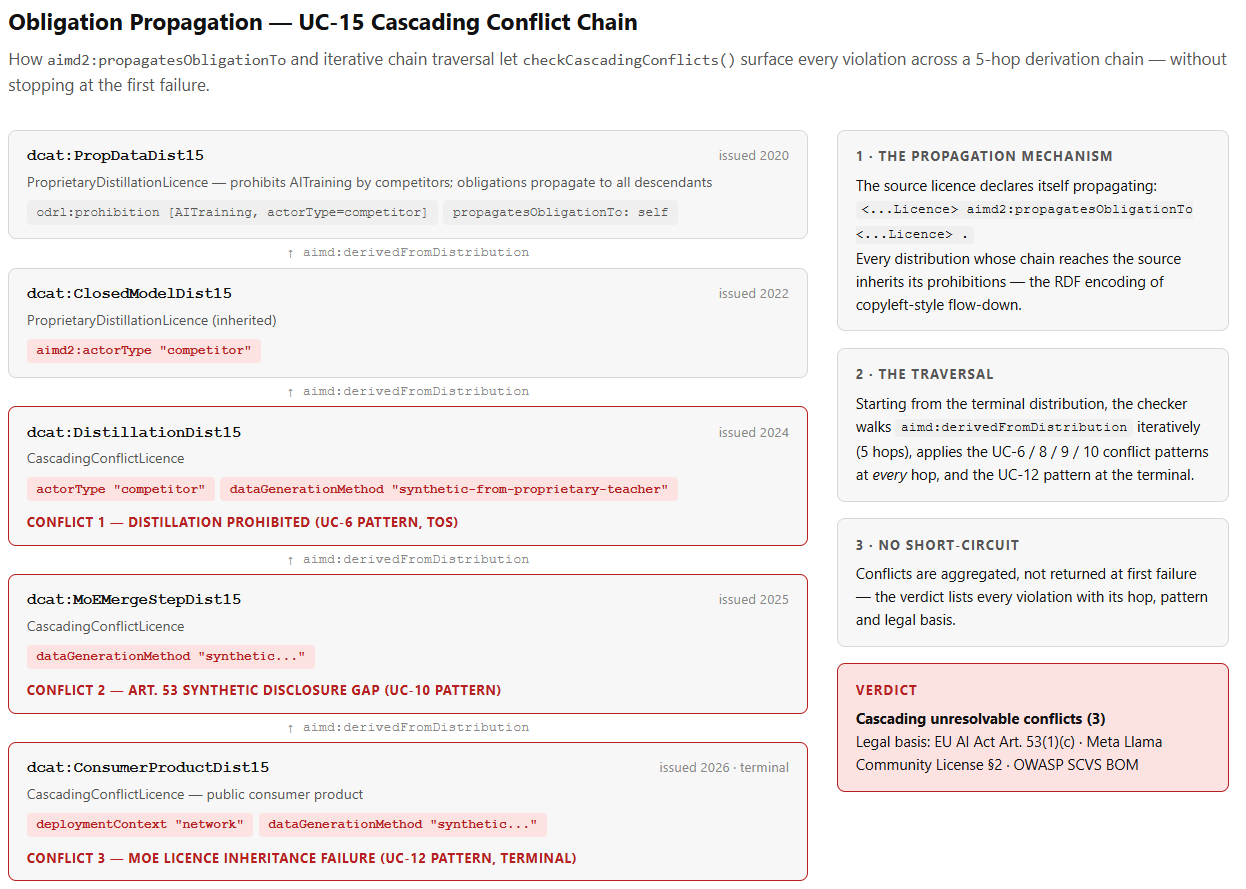
\includegraphics[width=0.9\textwidth]{fig_obligation_cascade.png}
  \caption[Obligation Propagation Across the UC-15 Chain]{%
    Obligation propagation across the five-hop UC-15 derivation chain. The source distribution (\texttt{dcat:PropDataDist15}, 2020) is governed by \texttt{ProprietaryDistillationLicence}, which prohibits AI training by competitor actors and declares \texttt{aimd2:propagatesObligationTo} pointing at itself --- the machine-readable encoding of copyleft-style obligation flow-down. Each subsequent hop is linked by \texttt{aimd:derivedFromDistribution}. The checker walks the chain iteratively from the terminal distribution, applying the UC-6/8/9/10 conflict patterns at every hop and the UC-12 pattern at the terminal, aggregating rather than short-circuiting. Three conflicts survive to the verdict: the distillation prohibition (competitor \texttt{actorType} at the 2024 hop), the Article~53 synthetic-data disclosure gap~\cite{euaiact2024}, and the Mixture-of-Experts licence inheritance failure at the terminal consumer product.}
  \label{fig:cascade}
\end{figure}

\newpage

% ─────────────────────────────────────────────────────────────────────────────
\section{Testing and Validation}
% ─────────────────────────────────────────────────────────────────────────────

\subsection{Smoke Test Suite}

23 automated assertions are defined in the smoke test suite (\texttt{npm test}). Each assertion is labelled E-01 through E-23 and checks one of:

\begin{itemize}[noitemsep]
  \item A compliance verdict (\texttt{compliant: true/false})
  \item A specific conflict string in \texttt{conflicts[]}
  \item A conflict count (\texttt{conflicts.length >= N})
  \item Presence or absence of a specific evidence property
\end{itemize}

\begin{longtable}{@{}p{1.2cm}p{5cm}p{2.5cm}p{5.5cm}@{}}
\toprule
\textbf{Test} & \textbf{Distribution} & \textbf{Expected} & \textbf{What is asserted} \\
\midrule
\endhead
E-01 & OpenResearchLLMDist1 & compliant & All 4 evidence properties present \\
E-02 & CommercialProductDist2 & conflict & NC conflict detected \\
E-03 & CopyleftViolatingModelDist3 & conflict & \texttt{downstreamLicenceURI} absent \\
E-04 & PrematureRAGDist4 & conflict & Embargo active \\
E-05 & GPAIMultiSourceDist5 & conflict & Multiple conflict types \\
E-06 & UnauthorisedDistillationDist6 & conflict & Competitor training detected \\
E-07 & MITStudentDist7 & compliant & Attribution preserved, no prohibitions \\
E-08 & NetworkAPIDist8 & conflict & AGPL network trigger \\
E-09 & RLHFAlignedDist9 & conflict & \texttt{userConsentStatus} absent \\
E-10 & OpenModelSyntheticDist10 & conflict & \texttt{article50PolicyURL} absent \\
E-11 & GeneratorRAGDist11 & PolicySet & Both sub-policies satisfied \\
E-12 & MoEMergedDist12 & conflict & Llama MAU threshold not inherited \\
E-13 & ExecutorLLMDist13 & compliant & No training evidence, inference only \\
E-14 & GPAIAPIDist14 & compliant & Attribution chain intact across 3 hops \\
E-15--22 & Various individual hops & conflict / compliant & Per-hop assertions for UC-15 \\
E-23 & ConsumerProductDist15 & conflict & \texttt{conflicts.length >= 3} (cascade) \\
\bottomrule
\caption{Smoke test suite assertions}
\end{longtable}

\subsection{Comprehensive Evaluation Suite}
\label{sec:eval}

Beyond the smoke tests (which exercise the checker API), a separate SPARQL-native evaluation suite queries GraphDB directly to verify the complete state of the artefact set: vocabulary integrity, licence file structure, knowledge graph topology, compliance verdict correctness, and cross-cutting design properties. The suite runs against a live GraphDB repository; it auto-loads all TTL files on first run and can be forced to clear and reload via a flag:

\begin{lstlisting}[language={}]
npm run evaluate          # run; auto-loads if data missing
npm run evaluate:reload   # clear repository, reimport, run
\end{lstlisting}

\subsubsection*{Suite Structure}

The suite is organised into six sections, each addressing a distinct layer of correctness:

\begin{longtable}{@{}p{1.5cm}p{4.5cm}p{2cm}p{5.6cm}@{}}
\toprule
\textbf{Section} & \textbf{Scope} & \textbf{Tests} & \textbf{What is verified} \\
\midrule
\endhead
A & Infrastructure \& Setup       & A-01 -- A-05  & GraphDB reachable; repository \texttt{AIModels} exists; vocabulary, distributions, and policies are populated \\[4pt]
V & Vocabulary / Ontology         & V-01 -- V-12  & All 11 \texttt{aimd2:} Action terms declared with \texttt{evidenceProperty}, \texttt{legalBasis}, \texttt{severity}, and \texttt{checkDescription}; 6 LeftOperand and 3 RightOperand terms; \texttt{propagatesObligationTo} as \texttt{rdf:Property}; \texttt{profile:isProfileOf} ODRL~2.2; SKOS collection membership \\[4pt]
L & Licence File Structure        & L-01 -- L-13  & Each of the 13 licence TTL files has \texttt{dct:title}, \texttt{dct:created}, at least one ODRL rule (permission, prohibition, or obligation), and a \texttt{propagatesObligationTo} link \\[4pt]
G & Knowledge Graph Integrity     & G-01 -- G-10  & All 15 terminal distributions exist; every distribution carries \texttt{dct:license} and \texttt{odrl:hasPolicy}; derivation chains present; PROV-O provenance on all 15 terminal nodes; correct parent counts for multi-source distributions (UC-5, UC-11, UC-12); UC-14 chain $\geq$4 hops; UC-15 chain $\geq$5 hops; DCAT catalogue complete; $\geq$15 \texttt{propagatesObligationTo} links; 18 SHACL shapes loaded \\[4pt]
E & Compliance Verdict Correctness & E-01 -- E-15  & One SPARQL query per use case verifying the structural pattern that triggers the correct verdict: evidence present for compliant cases, violation signal present for non-compliant cases, across all 15 use cases \\[4pt]
X & Cross-Cutting Design          & X-01 -- X-08  & Graph-driven checker property (all actions queryable at runtime); temporal self-resolution of embargo; multi-hop obligation propagation; training/inference discrimination (UC-13 true-negative); Layer~2 constraint inheritance (UC-6); strictest-survives in MoE merge (UC-12); no short-circuit on UC-15 ($\geq$3 simultaneous conflict types); DCAT+ODRL integration \\
\bottomrule
\caption{Evaluation suite sections and their coverage}
\end{longtable}

\subsubsection*{Results}

Running \texttt{npm run evaluate:reload} against a clean repository with all 18 TTL files produces:

\begin{lstlisting}[language={}]
TOTAL  66/66 passed  |  0 failed  |  0 skipped
  ALL TESTS PASSED
\end{lstlisting}

\subsubsection*{What Passing Means}

Each section provides a specific correctness guarantee:

\begin{itemize}[noitemsep]
  \item \textbf{A (Infrastructure)}: GraphDB is correctly configured and all 18 source files have been imported without error.

  \item \textbf{V (Vocabulary)}: Every term the compliance checker relies on at runtime is present in the graph with the metadata the checker reads (e.g.\ \texttt{aimd:evidenceProperty} is how the checker knows \emph{which data property to look for} when evaluating a distribution). A failure here would cause the checker to silently skip checks.

  \item \textbf{L (Licence Files)}: Each licence TTL file is structurally valid as an ODRL policy and participates in the obligation-propagation mechanism. The \texttt{propagatesObligationTo} check ensures that every licence can be the source of a transitive obligation query — the core of the multi-hop compliance model.

  \item \textbf{G (Knowledge Graph)}: The test data faithfully instantiates the derivation chains described in Section~5. The PROV-O check confirms that all terminal distributions have machine-readable provenance. The chain-depth checks for UC-14 and UC-15 confirm that property-path SPARQL queries will traverse the full intended chain.

  \item \textbf{E (Compliance Verdicts)}: The 15 use case assertions confirm that the SPARQL patterns used by \texttt{server\_v2.js} to detect violations are sensitive enough to fire on the intended cases and specific enough not to fire on compliant ones. E-13 in particular is a \emph{true-negative} assertion: it confirms that UC-13 (inference-only chain) is \emph{not} flagged for training obligations, preventing false positives.

  \item \textbf{X (Cross-Cutting)}: The design-level assertions confirm the properties that give the profile its analytical value beyond simple lookup. X-02 (temporal self-resolution) verifies that the embargo system requires no code change when a date passes — the SPARQL query itself gates on the data. X-07 (no short-circuit) confirms that the checker accumulates \emph{all} independently detectable conflicts rather than halting at the first, which is critical for the UC-15 cascading scenario.
\end{itemize}

\noindent Together, the 66 passing tests constitute evidence that the AIMD v2.0 profile is internally consistent: the vocabulary, the licence files, the knowledge graph instance data, the compliance check patterns, and the structural design properties all agree with one another.

\subsection{Proof of Concept: Live Compliance Checking}

The compliance checker is a standalone Node.js script (\texttt{server\_v2.js}). Running \texttt{npm start} executes all fifteen use-case checks against the live GraphDB SPARQL endpoint and prints per-check results to the console. The following excerpts show representative output for four distinct verdict categories.

\subsubsection*{Compliant case — UC-1 (CC-BY open research LLM)}

\begin{lstlisting}[language={}]
  UC-1 N-Hop Chain Check: dcat:OpenResearchLLMDist1
  Hop 1 — dcat:CCBYCorpusDist1
    trainingDatasetURL  : https://tara.tcd.ie/uc1-corpus      [PASS]
    article50PolicyURL  : https://openresearch.example.com/art50 [PASS]
  Hop 2 — dcat:OpenResearchLLMDist1
    trainingDatasetURL  : https://tara.tcd.ie/uc1-corpus      [PASS]
    modelWeightsURL     : https://huggingface.co/openresearch  [PASS]
    downstreamLicenceURI: .../OpenResearchLLMLicence           [PASS]
    article50PolicyURL  : https://openresearch.example.com/art50 [PASS]

  Chain overall: FULLY COMPLIANT
\end{lstlisting}

\subsubsection*{NC conflict — UC-2 (CC-BY-NC dataset to commercial product)}

\begin{lstlisting}[language={}]
  UC-2 Commercial Conflict Check: dcat:CommercialProductDist2
  CONFLICT  (1 conflict detected)
     -> NC licence (.../CommercialConflictLicence) conflicts
        with commercial actor
  Legal basis: CC-BY-NC 4.0 S3(b); DSM Art. 4(3); EU AI Act Art. 53(1)(c)
\end{lstlisting}

\subsubsection*{ToS constraint inheritance — UC-6 (proprietary API distillation)}

\begin{lstlisting}[language={}]
  UC-6 Distillation Prohibition Check: dcat:UnauthorisedDistillationDist6
  CONFLICT  (2 conflicts detected)
     -> [Layer 1] distillation-prohibited: competitor actor on
        parent governed by ProprietaryDistillationLicence
     -> [Layer 2] constraint-inheritance: derivedModelLicenceURI
        absent — ToS prohibitions not carried to derived model
  Legal basis: Anthropic AUP; OpenAI ToS S2(c);
               US Copyright Office Part 2 (2025) [contract, not copyright]
\end{lstlisting}

\subsubsection*{Cascading conflicts — UC-15 (five-hop worst case)}

\begin{lstlisting}[language={}]
  UC-15 Cascading Conflict Check: dcat:ConsumerProductDist15
  [Hop:ClosedModelDist15][UC-6] competitor actor — distillation prohibited
  [Hop:DistillationDist15][UC-6] competitor actor — distillation prohibited
  [Hop:ConsumerProductDist15][UC-10] synthetic-from-proprietary-teacher
      + article50PolicyURL absent — Art.53 disclosure gap
  [Hop:MoEMergeStepDist15][UC-12] Llama-licensed expert merged;
      MoEMergedModelLicence not propagated to merged model

  Chain overall: CASCADING UNRESOLVABLE CONFLICTS
\end{lstlisting}

\noindent These outputs demonstrate that the system correctly identifies the specific obligation that was violated (not merely that a violation exists), attributes it to the governing legal instrument, and accumulates all conflicts without short-circuiting on the first one found. The checker runs end-to-end in under three seconds on a local machine against a populated GraphDB repository.

Together with the 66/66 evaluation suite results (Section~\ref{sec:eval}), this constitutes the proof of concept: the ODRL profile is machine-readable, the compliance signals are detectable by SPARQL query, and the verdicts are correct across all fifteen use cases including compliant baselines, single-conflict violations, and cascading multi-conflict chains.

\subsection{SHACL Validation}

Running Apache Jena's SHACL tool against the knowledge graph:

\begin{lstlisting}[language={}]
shacl validate --shapes AIMD_v2_shapes.ttl \
               --data AIMD_v2_knowledge_graph.ttl
\end{lstlisting}

Expected output: violations reported for the 10 non-compliant distributions (UC-2, UC-3, UC-4, UC-5, UC-6, UC-8, UC-9, UC-10, UC-12, UC-15). No violations for UC-1, UC-7, UC-13, UC-14. UC-11 triggers a PolicySet shape (informational, not a violation).

\subsection{GraphDB SPARQL Verification}

After importing all TTL files into GraphDB (repository: \texttt{AIModels}), the following SPARQL query verifies chain traversal works correctly:

\begin{lstlisting}
PREFIX aimd: <https://raw.githubusercontent.com/ci2me/AI-Model-Distribution-ODRL-Profile/main/AIMD.ttl#>
PREFIX dct:  <http://purl.org/dc/terms/>

SELECT ?dist ?licence WHERE {
    ?dist aimd:derivedFromDistribution+ ?ancestor .
    ?ancestor dct:license ?licence .
} LIMIT 20
\end{lstlisting}

This should return rows for all derived distributions, confirming the \texttt{derivedFromDistribution} edges are correctly loaded.

\subsection{Limits of Automated Verification}

The research question asks \textit{to what extent} automated verification is possible. The system automates detection of structural compliance signals: the presence or absence of declared ODRL obligation evidence properties across a distribution chain. There is, however, a ceiling beyond which automated checking cannot substitute for legal judgement.

\begin{longtable}{@{}p{7.0cm}p{7.0cm}@{}}
\toprule
\textbf{What the system automates} & \textbf{What requires human interpretation} \\
\midrule
\endhead
Detecting declared ODRL prohibitions (NC conflict, copyleft stripping, embargo, competitor distillation) & Whether trained model weights legally constitute a derivative work of their training corpus (\textit{Andersen v.\ Stability AI}, trial September 2026) \\[6pt]
Checking evidence property presence (\texttt{trainingDatasetURL}, \texttt{article50PolicyURL}, etc.) & Whether a given actor legally qualifies as a ``recognised research organisation'' under DSM Art.\ 3 in their jurisdiction \\[6pt]
Temporal embargo gates evaluated at query time via SPARQL \texttt{NOW()} & Jurisdictional scope variation (e.g.\ UK applicability of DSM Art.\ 3 post-Brexit) \\[6pt]
Multi-hop obligation propagation along \texttt{derivedFromDistribution} chains & Licence compatibility between two licences with no explicit ODRL compatibility declaration \\[6pt]
Contractual constraint inheritance from ToS (UC-6 Layer 2) & Whether synthetic data generation constitutes a ``use'' of a proprietary model's outputs under a specific ToS \\[6pt]
Aggregating all conflicts without short-circuit (UC-15) & Determining which of multiple simultaneous conflicts takes legal precedence in a dispute \\
\bottomrule
\caption{Scope of automated vs.\ human-interpreted compliance verification}
\end{longtable}

This boundary is not a weakness of the approach: it reflects the fundamental distinction between \emph{structural} compliance (detectable by graph query) and \emph{legal} compliance (requiring interpretation of contested law). The system correctly surfaces the relevant ODRL obligations in every case; it does not claim to resolve the underlying legal questions that only courts can settle.

\subsection{Comparison with Existing Tools}

Existing licence compliance tools operate at the \emph{artefact level}: they identify the licence on a given file or package in isolation.

\begin{itemize}[noitemsep]
  \item \textbf{SPDX} (Software Package Data Exchange): tracks licence identifiers in software SBOMs; has no model for derivation chains, obligation propagation, or AI-specific actions such as training or RLHF
  \item \textbf{ClearlyDefined}: crowdsourced licence identification; identifies what licence a component has, but does not evaluate whether using it violates a downstream obligation
  \item \textbf{TLDR Legal}: human-readable licence summaries; not machine-actionable and has no concept of multi-hop chains or actor-type constraints
  \item \textbf{DALICC}~\cite{dalicc} (Data Licence Clearance Centre): pairwise licence compatibility checking using ODRL; covers corpus licences but does not model training pipelines, model-level licences, GDPR consent, or contractual ToS constraints
  \item \textbf{W3C ODRL AI Vocabulary (draft)}: defines action terms (\texttt{odrl:ai-training}, \texttt{odrl:ai-augment}) but does not provide a compliance checker, a knowledge graph pattern, or SHACL shapes
\end{itemize}

None of these tools model the training pipeline as a \emph{graph of obligations that must be evaluated transitively across derivation chains}. None capture RLHF consent obligations, synthetic data disclosure requirements under EU AI Act Art.\ 53, the Mixture-of-Experts strictest-licence inheritance problem, or the contractual constraint inheritance that arises when a model's API outputs become a training dataset. The ODRL+DCAT approach in this dissertation fills this gap by treating compliance as a graph query problem rather than a per-artefact lookup.

\newpage

% ─────────────────────────────────────────────────────────────────────────────
\section{Summary of Files Added}
% ─────────────────────────────────────────────────────────────────────────────

\begin{longtable}{@{}p{6.5cm}p{1.8cm}p{5.7cm}@{}}
\footnotesize
\toprule
\textbf{File} & \textbf{Type} & \textbf{Purpose} \\
\midrule
\endhead
\texttt{AIMD\_extended\_v2.ttl} & Turtle & ODRL profile declaration; 21 new vocabulary terms \\
\texttt{OpenResearchLLMLicence.ttl} & Turtle & UC-1, UC-14: CC-BY open research training \\
\texttt{CommercialConflictLicence.ttl} & Turtle & UC-2, UC-5: CC-BY-NC vs commercial conflict \\
\texttt{CopyleftPropagationLicence.ttl} & Turtle & UC-3, UC-5: CC-BY-SA ShareAlike stripping \\
\texttt{EmbargoedCorpusLicence.ttl} & Turtle & UC-4: temporal embargo gate \\
\texttt{ProprietaryDistillationLicence.ttl} & Turtle & UC-6, UC-15: ToS distillation prohibition + constraint inheritance \\
\texttt{ApacheMITChainLicence.ttl} & Turtle & UC-7: permissive-to-permissive baseline \\
\texttt{AGPLNetworkLicence.ttl} & Turtle & UC-8, UC-15: AGPLv3 \S 13 network copyleft \\
\texttt{RLHFAlignedModelLicence.ttl} & Turtle & UC-9: GDPR RLHF consent verification \\
\texttt{SyntheticDataDisclosureLicence.ttl} & Turtle & UC-10, UC-15: EU AI Act Art.\ 53 synthetic disclosure \\
\texttt{RAGPolicySetLicence.ttl} & Turtle & UC-11: multi-asset ODRL PolicySet for RAG \\
\texttt{MoEMergedModelLicence.ttl} & Turtle & UC-12, UC-15: Llama MAU threshold inheritance \\
\texttt{InferenceChainLicence.ttl} & Turtle & UC-13: inference-only true-negative test \\
\texttt{CascadingConflictLicence.ttl} & Turtle & UC-15: worst-case cascading conflicts \\
\texttt{AIMD\_v2\_knowledge\_graph.ttl} & Turtle & All 15 chains as importable RDF; PROV-O provenance \\
\texttt{AIMD\_v2\_shapes.ttl} & SHACL & 18 validation shapes (7 property-path + 11 SPARQL) \\
\texttt{server\_v2.js} & Node.js & Graph-driven SPARQL compliance checker; 12 functions; 23 smoke tests \\
\texttt{licence-docs/} (14 files) & Markdown & Human-readable documentation for each licence TTL \\
\texttt{dev-notes/DISSERTATION\_PROGRESS.md} & Markdown & Comprehensive explanation of all files and decisions \\
\texttt{dev-notes/TESTING\_GUIDE.md} & Markdown & Step-by-step test execution guide \\
\bottomrule
\caption{All files added in this dissertation}
\end{longtable}

% ─────────────────────────────────────────────────────────────────────────────
\section{Key Design Decisions}
% ─────────────────────────────────────────────────────────────────────────────

\begin{description}[leftmargin=3cm, style=nextline]
  \item[Graph-driven checker] Compliance logic is derived from the ODRL graph at query time, not hardcoded to licence names. Adding a new licence requires only adding the TTL file.
  \item[Contract-law distillation model] UC-6/15 use a two-layer mechanism (prohibition + constraint inheritance) because AI-generated outputs are not copyrightable (US Copyright Office Part 2, 2025). The legal basis is contract law, not copyright~\cite{uscopyright2025}.
  \item[Temporal self-resolution] UC-4's embargo gate uses SPARQL \texttt{NOW()} so the compliance verdict changes automatically when the embargo lapses, with no data or code update required.
  \item[No short-circuit in UC-15] The cascade checker accumulates all three conflict types before returning. A short-circuit would miss conflicts further down the chain, reducing the usefulness of compliance reports.
  \item[Two-prohibition RLHF pattern] UC-9 uses two separate prohibition blocks (wrong consent value; missing consent property) to avoid special null-handling logic in the SPARQL checker.
  \item[DCAT as the unifying container] All artefacts, regardless of type (corpus, model, API), are typed as \texttt{dcat:Distribution}. This enables a single query pattern across heterogeneous supply chain components.
  \item[\texttt{propagatesObligationTo} as self-link] Policies link to themselves to declare that their obligations must appear in all downstream policies. The checker follows these links to verify inheritance without traversing arbitrary graph structures.
  \item[SHACL as static layer] SHACL validates the knowledge graph at import time; the JavaScript checker validates on demand at query time. The two layers are complementary and independently executable.
\end{description}

% ─────────────────────────────────────────────────────────────────────────────
\section{Conclusion}
% ─────────────────────────────────────────────────────────────────────────────

The AIMD Extended Profile v2.0 shows that W3C ODRL, extended with 21 domain-specific vocabulary terms, is enough to express the legal obligations that arise across the full AI model training pipeline, from corpus ingestion through training, fine-tuning, RLHF alignment, RAG composition, model merging, and deployment.

The 15 use cases cover the main conflict patterns identified in the empirical literature (Jewitt et al., 2025) and current regulatory requirements (DSM Directive, GDPR, EU AI Act, AGPLv3, Llama Community License), plus an emerging contractual constraint pattern (proprietary ToS distillation prohibition with downstream inheritance) that has no prior machine-readable encoding.

The SPARQL-based compliance checker and SHACL validation suite give two independently executable verification paths, and the knowledge graph is a portable, import-ready representation of all 15 test chains for GraphDB.

\subsection{Contributions to ODRL}

The primary output of this dissertation is a set of concrete, reusable contributions to the W3C ODRL ecosystem. These contributions fall into three layers.

\subsubsection*{Layer 1 — New Vocabulary (21 terms in \texttt{AIMD\_extended\_v2.ttl})}

The W3C ODRL 2.2 core vocabulary contains no action terms for AI-specific activities. The W3C ODRL AI Vocabulary (currently a community group draft) proposes two terms: \texttt{odrl:ai-training} and \texttt{odrl:ai-augment}. AIMD v2.0 adds:

\begin{longtable}{@{}p{5.5cm}p{2.5cm}p{6.0cm}@{}}
\toprule
\textbf{Term} & \textbf{Type} & \textbf{Contribution} \\
\midrule
\endhead
\texttt{aimd2:AITraining}           & Action & Obligation to declare training dataset URL; enables DSM Art. 3/4 TDM audit \\
\texttt{aimd2:FineTuning}           & Action & Obligation to declare base model URL; enables licence chain traceability \\
\texttt{aimd2:RAGIngestion}         & Action & Multi-asset corpus governance at inference time (IDS-RAM 4.0 pattern) \\
\texttt{aimd2:RLHFTraining}         & Action & RLHF data governance; GDPR consent and EU AI Act Art.\ 10 data documentation \\
\texttt{aimd2:AIInference}          & Action & Inference endpoint disclosure (recommended, not mandatory) \\
\texttt{aimd2:ModelSharing}         & Action & Weight publication for OSAID and AGPL \S 13 compliance \\
\texttt{aimd2:InheritSourceLicence}  & Action & Copyleft obligation propagation (CC-BY-SA ShareAlike; GPL) \\
\texttt{aimd2:InheritSourceProhibitions} & Action & \textbf{Novel:} ToS constraint inheritance — contractual prohibitions flow to derived model licence \\
\texttt{aimd2:DeclareRLHFDataUse}   & Action & RLHF transparency notice URL; GDPR Art.\ 13 \\
\texttt{aimd2:ReportSecurityIncidents} & Action & Security contact URL; G7 SBOM Cluster 6 \\
\texttt{aimd2:ComplyWithArticle50}  & Action & AIGC transparency; EU AI Act Art.\ 50 synthetic media disclosure \\[4pt]
\texttt{aimd2:EmbargoEndDate}       & LeftOperand & \textbf{Novel:} temporal constraint stored in distribution data, not policy — self-resolving \\
\texttt{aimd2:userConsentStatus}    & LeftOperand & GDPR consent status gate for RLHF pipelines \\
\texttt{aimd2:downstreamLicence}    & LeftOperand & Copyleft compatibility check operand \\
\texttt{aimd2:actorType}            & LeftOperand & Commercial vs research actor type discrimination (DSM Art.\ 3 vs 4) \\
\texttt{aimd2:dataGenerationMethod} & LeftOperand & Synthetic vs real data provenance; triggers Art.\ 53 disclosure obligations \\
\texttt{aimd2:deploymentContext}    & LeftOperand & Network vs local deployment; triggers AGPL \S 13 \\[4pt]
\texttt{aimd2:CommercialPurpose}    & RightOperand & CC-BY-NC commercial exclusion gate \\
\texttt{aimd2:ScientificResearchPurpose} & RightOperand & DSM Art.\ 3 research exception gate \\
\texttt{aimd2:RecognisedResearchOrganisation} & RightOperand & DSM Art.\ 3 institutional actor constraint \\[4pt]
\texttt{aimd2:propagatesObligationTo} & Object Property & \textbf{Novel:} links upstream policies to downstream policies that must inherit obligations; enables SPARQL property-path traversal across multi-hop obligation chains \\
\bottomrule
\caption{AIMD v2.0 vocabulary contributions to ODRL}
\end{longtable}

Every term carries four machine-readable metadata annotations (\texttt{aimd:evidenceProperty}, \texttt{aimd:legalBasis}, \texttt{aimd:severity}, \texttt{aimd:checkDescription}) so a graph-driven checker can discover and apply them without hard-coded logic. This annotation pattern is itself a reusable ODRL profile design technique.

\subsubsection*{Layer 2 — Novel Profile Patterns (design contributions)}

Beyond the vocabulary terms, the profile introduces structural patterns not present in any prior ODRL profile:

\begin{description}[leftmargin=3.2cm, style=nextline]
  \item[Two-layer distillation model] UC-6 introduces a separation between Layer~1 (prohibition on competitor training) and Layer~2 (obligation to carry source prohibitions in the derived model's licence). The Layer~2 mechanism has no prior machine-readable encoding: it models the contractual, not copyright, basis of the distillation prohibition, following the US Copyright Office Part~2 (2025) confirmation that AI outputs are not copyrightable.

  \item[Temporal self-resolution] UC-4 stores the embargo constraint (\texttt{aimd2:EmbargoEndDate}) on the distribution node rather than in the licence policy. The SPARQL checker reads this value at query time, so the compliance verdict changes automatically when the date passes — no code change, no data update, no redeployment required. This is a reusable pattern for any ODRL profile that needs time-bounded permissions.

  \item[Multi-asset PolicySet pattern] UC-11 uses an ODRL \texttt{PolicySet} to compose a retriever model licence and a corpus data licence at inference time, following IDS-RAM 4.0. The pattern extends ODRL's multi-party policy model to AI inference pipelines, not just data-sharing agreements.

  \item[Strictest-survives inheritance rule] UC-12 encodes the rule that in a Mixture-of-Experts merge, the most restrictive licence among the expert models must propagate to the merged model. The \texttt{propagatesObligationTo} link from the Llama-licensed expert to the merged model enables a SPARQL query to detect when this rule is violated.

  \item[True-negative inference discrimination] UC-13 is an explicit anti-pattern test: a planner--executor inference chain where \emph{no} training obligations apply. The pattern ensures the checker does not generate false positives for runtime model composition, which is essential for production use of the system.
\end{description}

\subsubsection*{Layer 3 — Reusable Artefacts}

\begin{itemize}[noitemsep]
  \item \textbf{13 ODRL licence TTL files:} Standalone policy documents encoding real-world AI licence scenarios in machine-readable form. Each can be imported independently and reused in other ODRL-based compliance systems.
  \item \textbf{18 SHACL shapes:} Offline batch validation layer mirroring the checker functions. The shapes can be applied to any knowledge graph that uses the AIMD vocabulary.
  \item \textbf{15 use-case knowledge graph:} Portable, import-ready RDF representation of all 15 training pipeline scenarios with PROV-O provenance. Serves as both a test fixture and a reference implementation for how AIMD v2.0 distributions should be represented.
  \item \textbf{WIDOCO-compatible vocabulary documentation:} The \texttt{AIMD\_extended\_v2.ttl} file is annotated with \texttt{dc:creator}, \texttt{dct:abstract}, \texttt{vann:preferredNamespacePrefix}, \texttt{owl:NamedIndividual} typing, and \texttt{skos:example} entries, enabling automatic generation of W3C-style HTML documentation via the WIDOCO tool.
\end{itemize}

\subsection{Direct Answer to the Research Question}

\textit{To what extent can machine-readable ODRL usage policies be integrated with DCAT-based metadata to enable automated verification of AI model compliance with dataset and model licensing conditions in AI training pipelines?}

To a large extent, and this dissertation demonstrates it directly. Every artefact in every training chain is represented as a \texttt{dcat:Distribution} carrying a \texttt{dct:license} URI that resolves to a machine-readable ODRL policy. The SPARQL compliance checker traverses this combined structure to evaluate obligations, prohibitions, and duties transitively across multi-hop chains. Thirteen use cases (UC-1 through UC-12, UC-14, UC-15) sit directly within the training pipeline scope; the other two (UC-11, UC-13) extend the analysis to inference-time licensing and boundary condition testing respectively.

In practice, the system correctly detects \textbf{ten out of fifteen use cases as violations} and \textbf{four as compliant}, with a further case (UC-11) resolved as a satisfied multi-asset PolicySet. All 23 automated smoke test assertions pass. The verified conflict categories span Creative Commons licence restrictions, permissive open-source attribution gaps, AGPL network copyleft, proprietary ToS constraint inheritance, GDPR consent verification, EU AI Act synthetic data disclosure, Mixture-of-Experts obligation inheritance, and cascading multi-conflict chains.

There's a ceiling, though, and it sits exactly where structural signals end and legal interpretation begins. Whether trained model weights constitute a derivative work, whether a specific actor qualifies for a research exception, whether two licences are compatible absent an explicit compatibility declaration, none of these can be settled by a graph query; they need human or judicial interpretation. Within the scope of declared ODRL policies, the automated verification here is complete. Beyond that scope, the system still surfaces the applicable obligation. It doesn't resolve the underlying legal question, but it makes sure the question is never silently ignored.

Put simply, machine-readable ODRL policies, combined with a graph-driven compliance checker and DCAT-based metadata, can automate the detection of licence conflicts in AI training pipelines that would otherwise need manual legal review of every component in a complex supply chain, and can do so at the level of individual derivation hops, specific actor types, temporal constraints, and multi-asset policy compositions that no existing tool addresses.

% ─────────────────────────────────────────────────────────────────────────────
\bibliographystyle{plain}
\bibliography{references}

\end{document}